%% Generated by Sphinx.
\def\sphinxdocclass{report}
\documentclass[a4paper,10pt,french]{book}
\ifdefined\pdfpxdimen
   \let\sphinxpxdimen\pdfpxdimen\else\newdimen\sphinxpxdimen
\fi \sphinxpxdimen=.75bp\relax

\PassOptionsToPackage{warn}{textcomp}
\usepackage[utf8]{inputenc}
\ifdefined\DeclareUnicodeCharacter
% support both utf8 and utf8x syntaxes
\edef\sphinxdqmaybe{\ifdefined\DeclareUnicodeCharacterAsOptional\string"\fi}
  \DeclareUnicodeCharacter{\sphinxdqmaybe00A0}{\nobreakspace}
  \DeclareUnicodeCharacter{\sphinxdqmaybe2500}{\sphinxunichar{2500}}
  \DeclareUnicodeCharacter{\sphinxdqmaybe2502}{\sphinxunichar{2502}}
  \DeclareUnicodeCharacter{\sphinxdqmaybe2514}{\sphinxunichar{2514}}
  \DeclareUnicodeCharacter{\sphinxdqmaybe251C}{\sphinxunichar{251C}}
  \DeclareUnicodeCharacter{\sphinxdqmaybe2572}{\textbackslash}
\fi
\usepackage{cmap}
\usepackage[T1]{fontenc}
\usepackage{amsmath,amssymb,amstext}
\usepackage{babel}
\usepackage{amsmath,amsfonts,amssymb,amsthm}
\usepackage{fncychap}
\usepackage{sphinx}
\sphinxsetup{hmargin={0.7in,0.7in}, vmargin={1in,1in},     verbatimwithframe=true,     TitleColor={rgb}{0,0,0},     HeaderFamily=\rmfamily\bfseries,     InnerLinkColor={rgb}{0,0,1},     OuterLinkColor={rgb}{0,0,1}}
\fvset{fontsize=\small}
\usepackage{geometry}

% Include hyperref last.
\usepackage{hyperref}
% Fix anchor placement for figures with captions.
\usepackage{hypcap}% it must be loaded after hyperref.
% Set up styles of URL: it should be placed after hyperref.
\urlstyle{same}

\addto\captionsfrench{\renewcommand{\figurename}{Fig.\@ }}
\makeatletter
\def\fnum@figure{\figurename\thefigure{}}
\makeatother
\addto\captionsfrench{\renewcommand{\tablename}{Tableau }}
\makeatletter
\def\fnum@table{\tablename\thetable{}}
\makeatother
\addto\captionsfrench{\renewcommand{\literalblockname}{Code source}}

\addto\captionsfrench{\renewcommand{\literalblockcontinuedname}{suite de la page précédente}}
\addto\captionsfrench{\renewcommand{\literalblockcontinuesname}{suite sur la page suivante}}
\addto\captionsfrench{\renewcommand{\sphinxnonalphabeticalgroupname}{Non-alphabetical}}
\addto\captionsfrench{\renewcommand{\sphinxsymbolsname}{Symboles}}
\addto\captionsfrench{\renewcommand{\sphinxnumbersname}{Numbers}}

\addto\extrasfrench{\def\pageautorefname{page}}

\setcounter{tocdepth}{1}


    %% %% %% %% %% %% %% %% %% %% Meher %% %% %% %% %% %% %% %% %%
    %% %add number to subsubsection 2=subsection, 3=subsubsection
    %% % below subsubsection is not good idea.
    \setcounter{secnumdepth}{3}
    %
    %% %% Table of content upto 2=subsection, 3=subsubsection
    \setcounter{tocdepth}{2}
    \usepackage{amsmath,amsfonts,amssymb,amsthm}
    \usepackage[bitstream-charter]{mathdesign}
    \usepackage{graphicx}
    %% % r educe spaces for Table of contents, figures and tables
    %% % i t is used "\addtocontents{toc}{\vskip -1.2cm}" etc. in the document
    \usepackage[notlot,nottoc,notlof]{}
    \usepackage{color}
    \usepackage{transparent}
    \usepackage{eso-pic}
    \usepackage{lipsum}
    \usepackage{footnotebackref} %% link at the footnote to go to the place of footnote in the text
    %% spacing between line
    \usepackage{setspace}
    %% %% \onehalfspacing
    %% %% \doublespacing
    \singlespacing
    %% %% %% %% %% % d atetime
    \usepackage{datetime}
    \newdateformat{MonthYearFormat}{%
    \monthname[\THEMONTH], \THEYEAR}
    %% RO, LE will not work for 'oneside' layout.
    %% Change oneside to twoside in document class
    \usepackage{fancyhdr}
    \pagestyle{fancy}
    \fancyhf{}
    %% % Alternating Header for oneside
    \fancyhead[L]{\ifthenelse{\isodd{\value{page}}}{ \small \nouppercase{\leftmark} }{}}
    \fancyhead[R]{\ifthenelse{\isodd{\value{page}}}{}{ \small \nouppercase{\rightmark} }}
    %% % Alternating Header for two side
    %\fancyhead[RO]{\small \nouppercase{\rightmark}}
    %\fancyhead[LE]{\small \nouppercase{\leftmark}}
    % for oneside: change footer at right side. If you want to use Left and right then use same as header defined above.
    \fancyfoot[R]{\ifthenelse{\isodd{\value{page}}}{{\tiny David THERINCOURT} }{}{\tiny Arduino}}
    %% % Alternating Footer for two side
    %\fancyfoot[RO, RE]{\scriptsize Meher Krishna Patel (mekrip@gmail.com)}
    %% % page number
    \fancyfoot[CO, CE]{\thepage}
    \renewcommand{\headrulewidth}{0.5pt}
    \renewcommand{\footrulewidth}{0.5pt}
    \RequirePackage{tocbibind} %% % c omment this to remove page number for following
    \addto\captionsenglish{\renewcommand{\contentsname}{Table of contents}}
    \addto\captionsenglish{\renewcommand{\listfigurename}{List of figures}}
    \addto\captionsenglish{\renewcommand{\listtablename}{List of tables}}
    % \addto\captionsenglish{\renewcommand{\chaptername}{Chapter}}
    %% reduce spacing for itemize
    \usepackage{enumitem}
    \setlist{nosep}
    %% %% %% %% %% % Quote Styles at the top of chapter
    \usepackage{epigraph}
    \setlength{\epigraphwidth}{0.8\columnwidth}
    \newcommand{\chapterquote}[2]{\epigraphhead[60]{\epigraph{\textit{#1}}{\textbf {\textit{--#2}}}}}
    %% %% %% %% %% % Quote for all places except Chapter
    \newcommand{\sectionquote}[2]{{\quote{\textit{``#1''}}{\textbf {\textit{--#2}}}}}
    %%%%%%%%%%%%%%%%%%%%%%%%%%%%%%%%%%%%
    \usepackage{xcolor}			
    \definecolor{bl}{rgb}{0.0,0.2,0.6}	%%% Bleu des titres
    \usepackage{sectsty}		
    %\allsectionsfont{\color{bl}\scshape\selectfont}
    \chapterfont{\color{bl}\rmfamily\centering}
    \partfont{\color{bl}\rmfamily\centering}
    \sectionfont{\color{bl}\rmfamily\raggedright}
    %\renewcommand{\thesection}{\Roman{section} -}
    \subsectionfont{\color{bl}\rmfamily\raggedright}
    %\renewcommand{\thesubsection}{\arabic{subsection})}
    \subsubsectionfont{\rmfamily\raggedright}
    %\renewcommand{\thesubsubsection}{\alph{subsubsection})}
    \paragraphfont{\rmfamily\raggedright}
    %\renewcommand{\theparagraph}{\alph{paragraph})}
    \subparagraphfont{\rmfamily\raggedright}
    %\renewcommand{\thesubparagraph}{\roman{subparagraph})}
    

\title{Microcontroleurs et sciences physiques}
\date{nov. 10, 2019}
\release{}
\author{THERINCOURT David}
\newcommand{\sphinxlogo}{\vbox{}}
\renewcommand{\releasename}{ }
\makeindex
\begin{document}

\ifdefined\shorthandoff
  \ifnum\catcode`\=\string=\active\shorthandoff{=}\fi
  \ifnum\catcode`\"=\active\shorthandoff{"}\fi
\fi

\pagestyle{empty}

    \pagenumbering{Roman} %% % to avoid page 1 conflict with actual page 1
    \begin{titlepage}
    \centering
    \vspace*{40mm} %% % * is used to give space from top
    \textbf{\Huge {Microcontrôleurs pour les sciences physiques}}
    \vspace{0mm}
    \begin{figure}[!h]
    \centering
    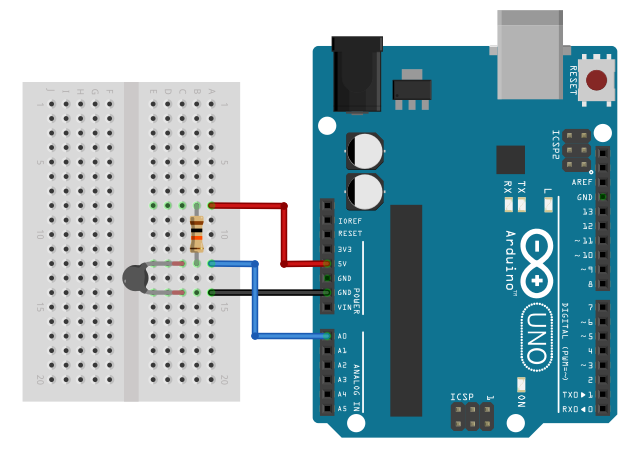
\includegraphics[scale=0.4]{CTN_Montage.png}
    \end{figure}
    \vspace{0mm}
    \\
    \Large \textbf{{David THERINCOURT}}
    \vspace*{0mm}
    \\
    \small 31 octobre 2019
    %% \vfill adds at the bottom
    \vfill
    \small \textit{Plus d'informations sur }{\href{https://physique.david-therincourt.fr/microcontroleurs/}{physique.david-therincourt.fr/microcontroleurs/}}
    \end{titlepage}
    \clearpage
    \pagenumbering{roman}
    \tableofcontents
    %\listoffigures
    %\listoftables
    \clearpage
    \pagenumbering{arabic}
    
\pagestyle{plain}
 
\pagestyle{normal}
\phantomsection\label{\detokenize{index::doc}}


Les nouveaux programmes 2019 en seconde générale et technologique, en première générale et en terminale générale introduisent l’utilisation des \sphinxstylestrong{microcontrôleurs} et des \sphinxstylestrong{capteurs} en sciences physiques.

Cette document a pour objectif d’apporter aux professeurs de physique-chimie les notions techniques nécessaires sur les microcontrôleurs afin d’aborder au mieux les nouvelles \sphinxstylestrong{capacités numériques}.


\chapter{Introduction aux microcontrôleurs}
\label{\detokenize{1_introduction/introduction:introduction-aux-microcontroleurs}}\label{\detokenize{1_introduction/introduction::doc}}

\section{Qu’est-ce qu’un microcontrôleur ?}
\label{\detokenize{1_introduction/introduction:qu-est-ce-qu-un-microcontroleur}}
Un microcontrôleur est un circuit intégré regroupant un micro-processeur, de la mémoire et des périphériques sur la même puce. Contrairement à un microprocesseur classique, un \sphinxstylestrong{microcontrôleur est surtout utilisé pour une application spécifique}.

De nos jours, les microcontrôleurs sont présents un peu partout : dans les appareils domestiques, médicaux, de télécommunication, dans les voitures, les avions, l’industrie, …

Apparus dans les années 70, les microcontrôleurs à architecture 8 bits ne sont pas près de disparaître. Très peu chère, on les retrouve dans des petites applications (ex. télécommande). Par exemple, la célèbre carte Arduino UNO fonctionne avec un microcontrôleur 8 bits !

\begin{figure}[H]
\centering
\capstart

\noindent\sphinxincludegraphics[width=400.00000\sphinxpxdimen,height=266.50000\sphinxpxdimen]{{Arduino_Uno_rev3_wikipedia}.jpg}
\caption{Carte Arduino UNO (microcontrôleur Atmel ATMEGA 328)}\label{\detokenize{1_introduction/introduction:id1}}\end{figure}

Actuellement, la tendance est aux microcontrôleurs 32 bits (ex. ARM Cortex-M, STM32, …) qui sont plus adaptés aux applications plus évoluées. C’est ce type de microcontrôleur qui a permis le portage du langage Python (MicroPython) au sein des microcontrôleurs. Les cartes Micro:bit, Pyboard ou encore à base d’ESP32 en sont les parfaits exemples !

\begin{figure}[H]
\centering
\capstart

\noindent\sphinxincludegraphics[width=400.00000\sphinxpxdimen,height=266.00000\sphinxpxdimen]{{microbit_flickr}.jpg}
\caption{Carte micro:bit}\label{\detokenize{1_introduction/introduction:id2}}\end{figure}

\begin{figure}[H]
\centering
\capstart

\noindent\sphinxincludegraphics[width=350.00000\sphinxpxdimen,height=350.00000\sphinxpxdimen]{{pyboard}.jpg}
\caption{Carte PyBoard (microcontrôleur STM32)}\label{\detokenize{1_introduction/introduction:id3}}\end{figure}

\begin{figure}[H]
\centering
\capstart

\noindent\sphinxincludegraphics[width=312.50000\sphinxpxdimen,height=240.00000\sphinxpxdimen]{{ESP-WROOM-32_Dev_Board}.jpg}
\caption{Carte ESP-WROOM-32 (microcontrôleur ESP32)}\label{\detokenize{1_introduction/introduction:id4}}\end{figure}


\section{Les différents types de microcontrôleurs}
\label{\detokenize{1_introduction/introduction:les-differents-types-de-microcontroleurs}}
Plusieurs critères permettent de différencier les microcontrôleurs : leur architecture, le nombre et le type de périphériques d’entrées/sorties, le langage de programmation, …

Ces deux derniers points sont à prendre en considération. En particulier, au lycée, le choix de Python comme langage de programmation des microcontrôleurs paraît logique.

En pratique, la plupart des manuels de sciences physiques et des fabricants de matériel spécialisé se sont tournés vers les populaires cartes Arduino même si le langage de programmation utilisé n’est pas du Python mais du C/C++ !


\section{Pourquoi des microcontrôleurs en sciences physiques}
\label{\detokenize{1_introduction/introduction:pourquoi-des-microcontroleurs-en-sciences-physiques}}
Le monde actuel est fortement imprégné par le numérique. Par exemple, les téléphones portables et les objets connectés comportent une \sphinxstylestrong{multitude de capteurs} mesurant des grandeurs très variées comme la température, la fréquence cardiaque, la pression, l’accélération, les ondes sonores, …

Il est donc important d’expliquer comment la valeur d’une \sphinxstylestrong{grandeur physique analogique} est obtenue sur un appareil numérique.

Il en est de même pour la génération de signaux (ex. son) à partir d’un appareil numérique.


\section{Que faire des microcontrôleurs en sciences physiques ?}
\label{\detokenize{1_introduction/introduction:que-faire-des-microcontroleurs-en-sciences-physiques}}
En sciences physiques, les microcontrôleurs peuvent-être utiliser pour :
\begin{itemize}
\item {} 
des \sphinxstylestrong{petites applications} (ex. thermomètre, télémètre à ultrasons, …) ou dans des \sphinxstylestrong{projets} en enseignement scientifique ;

\item {} 
\sphinxstylestrong{générer de signaux} (ex. génération d’un son, génération d’une commande, …) ;

\item {} 
\sphinxstylestrong{mesurer des durées} (ex. période, fréquence, temps caractéristique, …).

\end{itemize}

Mais il est également possible de :
\begin{itemize}
\item {} 
réaliser des \sphinxstylestrong{appareils de mesure programmables et modulables} (ex. pressionmètre, teslamètre, joulemètre, …) ;

\item {} 
faire de \sphinxstylestrong{l’acquisition de données} en mode \sphinxstylestrong{autonome} (ex. mesure de pression sur un ballon sonde) ou mode \sphinxstylestrong{connecté} (branché à un ordinateur).

\end{itemize}


\chapter{Les microcontrôleurs Arduino}
\label{\detokenize{2_arduino/index:les-microcontroleurs-arduino}}\label{\detokenize{2_arduino/index::doc}}

\section{Introduction}
\label{\detokenize{2_arduino/1_introduction:introduction}}\label{\detokenize{2_arduino/1_introduction::doc}}
\sphinxstylestrong{Arduino} est une \sphinxstylestrong{carte électronique} à base de microcontrôleur (ex. ATMEL AVR ATMEGA) développée par Arduino.cc sous licence libre. Tous les schémas des cartes sont disponibles librement sur le Web. A peu près une vingtaine de versions de cartes officielles ont été fabriquées dont la célèbre l’Arduino UNO.

\noindent{\hspace*{\fill}\sphinxincludegraphics[width=540\sphinxpxdimen,height=413\sphinxpxdimen]{{Arduino_boards_Arduino.cc}.png}\hspace*{\fill}}

A l’origine conçue pour la \sphinxstylestrong{création artistique}, la carte Arduino trouve des applications dans des domaines d’applications aussi variés qu’insolites. Une carte Arduino s’utilise généralement comme :
\begin{itemize}
\item {} 
\sphinxstylestrong{dispositif autonome} dans des applications comme la domotique, la robotique, les systèmes embarqués, …

\item {} 
\sphinxstylestrong{interface} entre un ordinateur (logiciel tiers) et des capteurs ou des actionneurs ;

\end{itemize}

\sphinxstylestrong{Arduino} est aussi le \sphinxstylestrong{logiciel de développement} des cartes du même nom. Également sous licence libre, cet environnement de développement intégré (IDE) utilise C/C++ comme langage de programmation et le port USB pour le téléversement du programme obtenu.


\section{Les cartes Arduino pour les sciences physiques}
\label{\detokenize{2_arduino/2_cartes_arduino:les-cartes-arduino-pour-les-sciences-physiques}}\label{\detokenize{2_arduino/2_cartes_arduino::doc}}

\subsection{La carte Arduino UNO (Rev 3)}
\label{\detokenize{2_arduino/2_cartes_arduino:la-carte-arduino-uno-rev-3}}
\noindent{\hspace*{\fill}\sphinxincludegraphics[width=400\sphinxpxdimen,height=255\sphinxpxdimen]{{Arduino_Uno_rev3_wikipedia1}.jpg}\hspace*{\fill}}

\sphinxstylestrong{Arduino UNO} est une des cartes officielles les plus récentes et économiques.

Caractéristiques principales :
\begin{itemize}
\item {} 
microcontroleur 8 bits ATMEGA328P cadencé à 16 Mhz ;

\item {} 
alimentation externe (7 à 12 V) ou USB (5 V);

\item {} 
programmation et communication via port USB ;

\item {} 
14 broches d’entrées/sorties numériques dont 6 PWM ;

\item {} 
6 entrées analogiques sur 10 bits ;

\item {} 
1 port I2C (communication avec capteurs/actionneurs numériques) ;

\item {} 
1 port UART (communication série) ;

\item {} 
3 timers (comptage et mesure de temps) ;

\item {} 
gestion des interruptions.

\end{itemize}

\noindent{\hspace*{\fill}\sphinxincludegraphics[width=336.00000\sphinxpxdimen,height=238.00000\sphinxpxdimen]{{arduino-uno_rev3_pixabay}.png}\hspace*{\fill}}

\begin{sphinxadmonition}{warning}{Avertissement:}
Les niveaux de tension acceptables sur les broches d’entrées doivent être \sphinxstylestrong{comprises entre 0 V et 5 V} sous peine de détruire le microcontrôleur ou la carte !
\end{sphinxadmonition}

\begin{sphinxadmonition}{note}{Note:}
La carte Arduino UNO ne possède pas de vraies sorties analogiques mais des sorties à \sphinxstylestrong{modulation de largeur d’impulsion} (MLI). Ce sont les six fameuses \sphinxstylestrong{sorties PWM} (Pulse Width Modulation).
\end{sphinxadmonition}


\subsection{Les cartes spécifiques pour les sciences physiques}
\label{\detokenize{2_arduino/2_cartes_arduino:les-cartes-specifiques-pour-les-sciences-physiques}}
Il s’agit de cartes spécialement concues pour les sciences physiques avec des \sphinxstylestrong{protections sur les ports d’entrée/sortie} contre les mauvaises manipulations (ce type de protections n’existe pas sur les cartes classiques comme l’Arduino Uno). Ces cartes disposent de leurs \sphinxstylestrong{propres capteurs} avec une connectique particulière.


\subsubsection{Educaduino Lab (Eurosmart)}
\label{\detokenize{2_arduino/2_cartes_arduino:educaduino-lab-eurosmart}}
\sphinxurl{https://educaduino-lab.com/}

\begin{figure}[H]
\centering
\capstart

\noindent\sphinxincludegraphics[width=400.00000\sphinxpxdimen,height=250.00000\sphinxpxdimen]{{Educaduino_Lab_DT}.jpg}
\caption{La carte Educaduino-Lab (E-LAB)}\label{\detokenize{2_arduino/2_cartes_arduino:id1}}\end{figure}

La carte \sphinxstylestrong{Educaduino Lab} a été concue sur la base d’une carte Arduino MEGA 2560. Cette dernière est équivalente à une carte arduino UNO mais avec plus de mémoire et surtout \sphinxstylestrong{plus de ports d’entrée/sortie}. Ce qui a permis à Eurosmart d’y placer des \sphinxstylestrong{connecteurs USB pour ses propres capteurs} tout en gardant la connectique classique de l’Arduino UNO.

Caractéristiques principales :
\begin{itemize}
\item {} 
microcontrôleur ATMEGA 2560 (comme l’Arduino MEGA 2560) ;

\item {} 
protection des ports d’entrée/sortie ;

\item {} 
brochage compatible Arduino Uno Rev 3 (pin 0.8mm, shield Grove, …) ;

\item {} 
ports supplémentaires en USB pour capteurs Educaduino-Lab ;

\end{itemize}

\begin{figure}[H]
\centering
\capstart

\noindent\sphinxincludegraphics[width=400.00000\sphinxpxdimen,height=242.00000\sphinxpxdimen]{{educaduino_manip_temperature}.png}
\caption{Mesure d’une température (image : Eurosmart)}\label{\detokenize{2_arduino/2_cartes_arduino:id2}}\end{figure}

Une malette avec un afficheur LCD et plusieurs capteurs adaptée au programme du lycée est également proposée.

\begin{figure}[H]
\centering
\capstart

\noindent\sphinxincludegraphics[width=400.00000\sphinxpxdimen,height=393.50000\sphinxpxdimen]{{educaduino_malette}.png}
\caption{Kit sciences-physiques 2nde/1ère (image : Eurosmart)}\label{\detokenize{2_arduino/2_cartes_arduino:id3}}\end{figure}


\subsubsection{Plug’Uino® Uno (Sciencéthic)}
\label{\detokenize{2_arduino/2_cartes_arduino:pluguino-uno-sciencethic}}
\sphinxurl{https://www.sciencethic.com/}

\begin{figure}[H]
\centering
\capstart

\noindent\sphinxincludegraphics[width=282.80000\sphinxpxdimen,height=260.40000\sphinxpxdimen]{{sciencethic_plugiuno_uno}.png}
\caption{La carte Plug’Uino ® Uno (image : Sciencéthic)}\label{\detokenize{2_arduino/2_cartes_arduino:id4}}\end{figure}

Sciencéthic propose également une carte \sphinxstylestrong{Plug’Uino Uno} protégée contre les mauvaises manipulations et 100\% compatible Arduino UNO Rev 3.

Caractéristiques principales :
\begin{itemize}
\item {} 
microcontrôleur ATMEGA 328P (comme l’Arduino Uno) ;

\item {} 
protection des ports d’entrée/sortie ;

\item {} 
brochage compatible Arduino Uno Rev 3 (pin 0.8mm, shield Grove, …) ;

\item {} 
connecteurs SATA pour les capteurs Plug’uino ;

\end{itemize}

\begin{figure}[H]
\centering
\capstart

\noindent\sphinxincludegraphics[width=336.70000\sphinxpxdimen,height=199.50000\sphinxpxdimen]{{sciencethic_pluguino_uno_pression}.png}
\caption{Capteur de pression et loi de Mariotte (image : Sciencéthic)}\label{\detokenize{2_arduino/2_cartes_arduino:id5}}\end{figure}


\section{Le logiciel Arduino}
\label{\detokenize{2_arduino/3_arduino_ide:le-logiciel-arduino}}\label{\detokenize{2_arduino/3_arduino_ide::doc}}
Le logiciel \sphinxstylestrong{Arduino} est un environnement intégré de développement (IDE) multiplaforme. Il est téléchargeable sur le site officiel \sphinxurl{http://www.arduino.cc/en/}

\noindent{\hspace*{\fill}\sphinxincludegraphics[width=350.00000\sphinxpxdimen,height=284.90000\sphinxpxdimen]{{Arduino_IDE}.png}\hspace*{\fill}}

\begin{sphinxadmonition}{note}{Note:}
Arduino.cc propose une \sphinxstylestrong{version Web} (\sphinxurl{https://create.arduino.cc/}) de son environnement de développement. Elle nécessite l’installation d’un plugin afin de programmer la carte par le port USB.
\end{sphinxadmonition}


\subsection{Choix du port de communication avec la carte Arduino}
\label{\detokenize{2_arduino/3_arduino_ide:choix-du-port-de-communication-avec-la-carte-arduino}}
\noindent{\hspace*{\fill}\sphinxincludegraphics[width=572.60000\sphinxpxdimen,height=242.90000\sphinxpxdimen]{{Arduino_IDE_Select_Port}.png}\hspace*{\fill}}

\begin{sphinxadmonition}{warning}{Avertissement:}
Pour programmer une carte Arduino, il est nécessaire de connectée cette dernière à l’ordinateur par l’intermédiaire d’un câble USB. Une fois le logiciel Arduino lancé, il est \sphinxstylestrong{impératif de  sélectionner le port série} donnant accès à la carte Arduino (ex. COM3). Sinon il ne sera pas possible de téléverser le futur programme.
\end{sphinxadmonition}


\subsection{Mise en œuvre d’un projet Arduino :}
\label{\detokenize{2_arduino/3_arduino_ide:mise-en-oeuvre-d-un-projet-arduino}}
\noindent{\hspace*{\fill}\sphinxincludegraphics[width=500\sphinxpxdimen,height=33\sphinxpxdimen]{{Arduino_IDE_Barre_Outils}.png}\hspace*{\fill}}

La mise en œuvre d’un projet Arduino s’effectue dans l’ordre suivant :
\begin{enumerate}
\def\theenumi{\arabic{enumi}}
\def\labelenumi{\theenumi .}
\makeatletter\def\p@enumii{\p@enumi \theenumi .}\makeatother
\item {} 
\sphinxstylestrong{Édition} du programme dans l’éditeur de l’interface ;

\item {} 
\sphinxstylestrong{Vérification} du programme (compilation) ;

\item {} 
\sphinxstylestrong{Téléversement} du programme ;

\item {} 
\sphinxstylestrong{Exécution} sur le carte Arduino (de façon autonome sans ordinateur).

\end{enumerate}


\section{Premier programme : Blink}
\label{\detokenize{2_arduino/4_exemple_blink:premier-programme-blink}}\label{\detokenize{2_arduino/4_exemple_blink::doc}}
Le programme \sphinxstylestrong{Blink} propose de faire clignoter la LED intégrée à la carte de développement (connectée sur la broche 13).


\subsection{Edition}
\label{\detokenize{2_arduino/4_exemple_blink:edition}}
Le programme \sphinxstylestrong{Blink} est disponible dans les exemples du logiciel \sphinxstylestrong{Arduino IDE}.

\begin{figure}[H]
\centering
\capstart

\noindent\sphinxincludegraphics[width=390.00000\sphinxpxdimen,height=302.50000\sphinxpxdimen]{{Blink_01_exemples_blink}.png}
\caption{Ouvrir le programme Blink}\label{\detokenize{2_arduino/4_exemple_blink:id1}}\end{figure}

\begin{figure}[H]
\centering
\capstart

\noindent\sphinxincludegraphics[width=375.00000\sphinxpxdimen,height=300.00000\sphinxpxdimen]{{Blink_02_edition_blink}.png}
\caption{Edition du programme Blink}\label{\detokenize{2_arduino/4_exemple_blink:id2}}\end{figure}

\begin{sphinxadmonition}{note}{Note:}\begin{itemize}
\item {} 
Un programme Arduino écrit en langage C/C++ est composé d’une suite d’intructions.

\item {} 
Ces instruction sont effectuées dans l’ordre des lignes de code.

\item {} 
Les \sphinxstylestrong{commentaires} en gris sont délimités par les caractères \sphinxcode{\sphinxupquote{/*}} et \sphinxcode{\sphinxupquote{*/}} sur plusieurs lignes ou commencent pas les caractères \sphinxcode{\sphinxupquote{//}} sur une même ligne.

\end{itemize}
\end{sphinxadmonition}

\begin{figure}[H]
\centering
\capstart

\noindent\sphinxincludegraphics[width=389.90000\sphinxpxdimen,height=366.10000\sphinxpxdimen]{{Blink_02_edition_blink_modifie}.png}
\caption{Une version modifiée du programme Blink}\label{\detokenize{2_arduino/4_exemple_blink:id3}}\end{figure}

\begin{sphinxadmonition}{warning}{Avertissement:}
Un progamme Arduino respecte toujours une \sphinxstylestrong{structure spécifique} composée en trois parties :
\begin{itemize}
\item {} 
Les déclarations : \sphinxstylestrong{définitions} des constantes et des variables ;

\item {} 
La fonction \sphinxcode{\sphinxupquote{setup()}} : \sphinxstylestrong{configuration} de la carte (entrées, sorties, port série, …) ;

\item {} 
La fonction \sphinxcode{\sphinxupquote{loop()}} : \sphinxstylestrong{instructions du programme exécutées} dans une \sphinxstylestrong{boucle infinie} (sans fin).

\end{itemize}
\end{sphinxadmonition}


\subsection{Compilation}
\label{\detokenize{2_arduino/4_exemple_blink:compilation}}
\begin{figure}[H]
\centering
\capstart

\noindent\sphinxincludegraphics[width=407.50000\sphinxpxdimen,height=300.00000\sphinxpxdimen]{{Blink_03_compilation_choix_carte}.png}
\caption{Choix du type de carte}\label{\detokenize{2_arduino/4_exemple_blink:id4}}\end{figure}

\begin{sphinxadmonition}{warning}{Avertissement:}
Avant de lancer la compilation, il est important de \sphinxstylestrong{choisir le modéle de carte Arduino utilisé}. Le programme généré est dépendant du type de microcontrôleur présent sur la carte.
\end{sphinxadmonition}

\begin{figure}[H]
\centering
\capstart

\noindent\sphinxincludegraphics[width=350.00000\sphinxpxdimen,height=420.00000\sphinxpxdimen]{{Blink_03_compilation_ksnip}.png}
\caption{Puis la compilation peut s’effectuée !}\label{\detokenize{2_arduino/4_exemple_blink:id5}}\end{figure}


\subsection{Téléversement}
\label{\detokenize{2_arduino/4_exemple_blink:televersement}}
\begin{figure}[H]
\centering
\capstart

\noindent\sphinxincludegraphics[width=427.50000\sphinxpxdimen,height=170.00000\sphinxpxdimen]{{Blink_04_televersement_choix_port}.png}
\caption{Choix du port de communication}\label{\detokenize{2_arduino/4_exemple_blink:id6}}\end{figure}

\begin{sphinxadmonition}{warning}{Avertissement:}
Pour téléverser le programme obtenu, il est nécessaire de \sphinxstylestrong{sélectionner le port de communication série} sur lequel est connectée la carte Arduino.
\end{sphinxadmonition}

\begin{figure}[H]
\centering
\capstart

\noindent\sphinxincludegraphics[width=350.00000\sphinxpxdimen,height=420.00000\sphinxpxdimen]{{Blink_04_televersement_ksnip}.png}
\caption{Téléversement du programme}\label{\detokenize{2_arduino/4_exemple_blink:id7}}\end{figure}


\subsection{Exécution}
\label{\detokenize{2_arduino/4_exemple_blink:execution}}
Le programme s’exécute sur la carte Arduino de façon autonome (sans ordinateur).

\begin{figure}[H]
\centering

\noindent\sphinxincludegraphics[width=280.00000\sphinxpxdimen,height=198.10000\sphinxpxdimen]{{Blink_05_execution_ksnip}.png}
\end{figure}


\section{Particularité du langage Arduino}
\label{\detokenize{2_arduino/5_particularite_langage:particularite-du-langage-arduino}}\label{\detokenize{2_arduino/5_particularite_langage::doc}}
Le langage de programmation C/C++ est utilisé par le logiciel Arduino pour programmer les microcontrôleurs Arduino.

\noindent{\hspace*{\fill}\sphinxincludegraphics[width=557\sphinxpxdimen,height=523\sphinxpxdimen]{{Blink_02_edition_blink_modifie}.png}\hspace*{\fill}}


\subsection{Syntaxe}
\label{\detokenize{2_arduino/5_particularite_langage:syntaxe}}\begin{itemize}
\item {} 
Toutes les instructions se terminent par un point virgule \sphinxcode{\sphinxupquote{;}} sauf pour les directives \sphinxcode{\sphinxupquote{\#include}} et \sphinxcode{\sphinxupquote{\#define}}.

\item {} 
Les blocs d’instructions sont délimités par des accolades \sphinxcode{\sphinxupquote{\{...\}}}.

\item {} 
Les \sphinxstylestrong{commentaires} en gris sont délimités par les caractères \sphinxcode{\sphinxupquote{/*}} et \sphinxcode{\sphinxupquote{*/}} sur plusieurs lignes ou commencent pas les caractères \sphinxcode{\sphinxupquote{//}} sur une même ligne.

\end{itemize}


\subsection{Typage des variables}
\label{\detokenize{2_arduino/5_particularite_langage:typage-des-variables}}
Le type d’une variable doit être renseigné à sa déclaration.

Quelques types disponibles :


\begin{savenotes}\sphinxattablestart
\centering
\begin{tabulary}{\linewidth}[t]{|T|T|T|}
\hline
\sphinxstyletheadfamily 
Type
&\sphinxstyletheadfamily 
Description
&\sphinxstyletheadfamily 
Valeurs
\\
\hline
\sphinxcode{\sphinxupquote{int}}
&
entier sur 16 bits
&
-32768 à 32767
\\
\hline
\sphinxcode{\sphinxupquote{long}}
&
entier sur 32 bits
&
-2147483648 à 2147483647
\\
\hline
\sphinxcode{\sphinxupquote{float}}
&
flottant sur 32 bits
&
-3.4028235E+38 à -3.4028235E+38 ;
\\
\hline
\sphinxcode{\sphinxupquote{char}}
&
caractère sur 8 bits
&
Table ASCII
\\
\hline
\end{tabulary}
\par
\sphinxattableend\end{savenotes}

Exemples :

\begin{sphinxVerbatim}[commandchars=\\\{\}]
\PYG{n+nb}{int} \PYG{n}{a} \PYG{o}{=} \PYG{l+m+mi}{5}\PYG{p}{;}
\PYG{n+nb}{float} \PYG{n}{pi} \PYG{o}{=} \PYG{l+m+mf}{3.14}\PYG{p}{;}
\PYG{n}{char} \PYG{n}{c} \PYG{o}{=} \PYG{l+s+s1}{\PYGZsq{}}\PYG{l+s+s1}{A}\PYG{l+s+s1}{\PYGZsq{}}\PYG{p}{;}
\end{sphinxVerbatim}


\subsection{Constantes prédéfinies}
\label{\detokenize{2_arduino/5_particularite_langage:constantes-predefinies}}
Afin d’améliorer la lecture du code, des constantes sont définies.


\begin{savenotes}\sphinxattablestart
\centering
\begin{tabulary}{\linewidth}[t]{|T|T|}
\hline
\sphinxstyletheadfamily 
Constante
&\sphinxstyletheadfamily 
Valeur
\\
\hline
\sphinxcode{\sphinxupquote{LOW}}
&
0 (niveau logique)
\\
\hline
\sphinxcode{\sphinxupquote{HIGH}}
&
1 (niveau logique)
\\
\hline
\sphinxcode{\sphinxupquote{OUTPUT}}
&
broche en sortie
\\
\hline
\sphinxcode{\sphinxupquote{INPUT}}
&
broche en entrée
\\
\hline
\sphinxcode{\sphinxupquote{LED\_BUILTIN}}
&
\sphinxcode{\sphinxupquote{13}} (numéro de broche de la LED intégrée)
\\
\hline
\end{tabulary}
\par
\sphinxattableend\end{savenotes}


\subsection{Structure du programme}
\label{\detokenize{2_arduino/5_particularite_langage:structure-du-programme}}
Un progamme Arduino respecte toujours une \sphinxstylestrong{structure spécifique} composée en trois parties :
\begin{itemize}
\item {} 
Les déclarations : \sphinxstylestrong{définitions} des constantes et des variables ;

\item {} 
La fonction \sphinxcode{\sphinxupquote{setup()}} : \sphinxstylestrong{configuration} de la carte (entrées, sorties, port série, …) ;

\item {} 
La fonction \sphinxcode{\sphinxupquote{loop()}} : \sphinxstylestrong{instructions du programme exécutées} dans une \sphinxstylestrong{boucle infinie} (sans fin).

\end{itemize}


\section{Pilotage d’une carte Arduino en Python avec Nanpy}
\label{\detokenize{2_arduino/6_nanpy:pilotage-d-une-carte-arduino-en-python-avec-nanpy}}\label{\detokenize{2_arduino/6_nanpy::doc}}

\subsection{Qu’est-ce que Nanpy ?}
\label{\detokenize{2_arduino/6_nanpy:qu-est-ce-que-nanpy}}
Nanpy est une librairie pour Python utilisée pour le \sphinxstylestrong{pilotage} d’une carte Arduino par le câble USB (port série).

\sphinxurl{https://nanpy.github.io/}


\subsection{Principe de fonctionnement}
\label{\detokenize{2_arduino/6_nanpy:principe-de-fonctionnement}}
La carte Arduino a été préalablement programmer avec le firmware \sphinxstylestrong{Nanpy} téléversé à partir du logiciel Arduino. Ce firmware est un \sphinxstylestrong{programme particulier} (écrit en langage Arduino C/C++) qui \sphinxstylestrong{gère le  protocole de communication} entre le programme Python exécuté sur l’ordinateur et la carte Arduino.

\begin{sphinxadmonition}{warning}{Avertissement:}
Il est important de retenir que \sphinxstylestrong{Nanpy ne permet pas un fonctionnement autonome} de la carte Arduino puisque le carte doit-être \sphinxstylestrong{constamment connectée à l’ordinateur} sur lequel le programme Python est exécuté !
\end{sphinxadmonition}


\subsection{Installation de firmware Nanpy sur une carte Arduino}
\label{\detokenize{2_arduino/6_nanpy:installation-de-firmware-nanpy-sur-une-carte-arduino}}

\subsubsection{Téléchargement du firmware}
\label{\detokenize{2_arduino/6_nanpy:telechargement-du-firmware}}
Le fichier \sphinxcode{\sphinxupquote{nanpy-firmware-master.zip}} est une librairie Arduino contenant le firmware Nanpy à installer sur la carte Arduino.

Ce fichier est à télécharger sur le site \sphinxurl{https://github.com/nanpy/nanpy-firmware}.

\noindent{\hspace*{\fill}\sphinxincludegraphics[width=499.00000\sphinxpxdimen,height=265.00000\sphinxpxdimen]{{nanpy_telechargement_firmware_ksnip}.png}\hspace*{\fill}}


\subsubsection{Installation du firmware dans le logiciel Arduino}
\label{\detokenize{2_arduino/6_nanpy:installation-du-firmware-dans-le-logiciel-arduino}}
Le fichier \sphinxcode{\sphinxupquote{nanpy-firmware-master.zip}} est à installer dans les librairies d’Arduino à partir du menu \sphinxtitleref{Croquis \textgreater{} Inclure une bibliothèque \textgreater{} Ajouter la bibliothèque au format .Zip …}

\noindent{\hspace*{\fill}\sphinxincludegraphics[width=375.00000\sphinxpxdimen,height=200.00000\sphinxpxdimen]{{nanpy_ajouter_librairie_ksnip}.png}\hspace*{\fill}}


\subsubsection{Téléversement du firmware dans la carte Arduino}
\label{\detokenize{2_arduino/6_nanpy:televersement-du-firmware-dans-la-carte-arduino}}
Ouvrir le fichier d’exemple \sphinxcode{\sphinxupquote{Nampy}} à partir du menu :

\sphinxstyleemphasis{Fichier \textgreater{} Exemples \textgreater{} nanpy-firmware-master \textgreater{} Nanpy}

\noindent{\hspace*{\fill}\sphinxincludegraphics[width=340.00000\sphinxpxdimen,height=420.00000\sphinxpxdimen]{{nanpy_ouvrir_exemple_ksnip}.png}\hspace*{\fill}}

Puis \sphinxstylestrong{téléverser} le programme dans la carte Arduino.

\noindent{\hspace*{\fill}\sphinxincludegraphics[width=350.00000\sphinxpxdimen,height=394.10000\sphinxpxdimen]{{nanpy_televersement_ksnip}.png}\hspace*{\fill}}

\begin{sphinxadmonition}{warning}{Avertissement:}
Ne pas oublier de sélectionner le type de carte (ex. Arduino Uno) et le port de communication série (ex. COM3) dans le menu \sphinxstyleemphasis{Outils} avant le téléversement du firmware !
\end{sphinxadmonition}

La carte est mainteanant prête pour un fonctionnement avec Nanpy !


\subsection{Installer la libairie Nanpy sur l’ordinateur}
\label{\detokenize{2_arduino/6_nanpy:installer-la-libairie-nanpy-sur-l-ordinateur}}
L’installation dépend de la distribution Python utilisée sur l’ordinateur.


\subsubsection{Pour EduPython}
\label{\detokenize{2_arduino/6_nanpy:pour-edupython}}
\sphinxurl{https://edupython.tuxfamily.org/}

Il n’y a rien à faire car la librairie Nanpy est installée par défaut.


\subsubsection{Pour les autres distributions}
\label{\detokenize{2_arduino/6_nanpy:pour-les-autres-distributions}}
Il faut installer manuellement à partir du dépôt internet \sphinxcode{\sphinxupquote{Pypi}} (\sphinxurl{https://pypi.org/project/nanpy/}) à l’aide de la commande \sphinxcode{\sphinxupquote{pip}} :

\begin{sphinxVerbatim}[commandchars=\\\{\}]
\PYG{n}{pip} \PYG{n}{install} \PYG{n}{nanpy}
\end{sphinxVerbatim}


\subsection{Exemple : Blink}
\label{\detokenize{2_arduino/6_nanpy:exemple-blink}}
Voici un exemple du programme \sphinxstylestrong{Blink} en Python.

\begin{sphinxVerbatim}[commandchars=\\\{\}]
\PYG{k+kn}{from} \PYG{n+nn}{nanpy} \PYG{k}{import} \PYG{n}{ArduinoApi}           \PYG{c+c1}{\PYGZsh{} Librairie du gestion des carte Arduino}
\PYG{k+kn}{from} \PYG{n+nn}{nanpy} \PYG{k}{import} \PYG{n}{SerialManager}        \PYG{c+c1}{\PYGZsh{} Librairie de gestion du port série}
\PYG{k+kn}{from} \PYG{n+nn}{time} \PYG{k}{import} \PYG{n}{sleep}                 \PYG{c+c1}{\PYGZsh{} Importation fonction sleep()}

\PYG{n}{port} \PYG{o}{=} \PYG{n}{SerialManager}\PYG{p}{(}\PYG{p}{)}                 \PYG{c+c1}{\PYGZsh{} Déclaration du port série}
\PYG{n}{uno} \PYG{o}{=} \PYG{n}{ArduinoApi}\PYG{p}{(}\PYG{n}{connection}\PYG{o}{=}\PYG{n}{port}\PYG{p}{)}      \PYG{c+c1}{\PYGZsh{} Déclaration de la carte Arduino Uno}

\PYG{n}{pinLed} \PYG{o}{=} \PYG{l+m+mi}{13}                            \PYG{c+c1}{\PYGZsh{} Led intégrée branchée sur boche 13}
\PYG{n}{uno}\PYG{o}{.}\PYG{n}{pinMode}\PYG{p}{(}\PYG{n}{pinLed}\PYG{p}{,}\PYG{n}{uno}\PYG{o}{.}\PYG{n}{OUTPUT}\PYG{p}{)}         \PYG{c+c1}{\PYGZsh{} Broche Led en sortie}

\PYG{k}{while} \PYG{k+kc}{True}\PYG{p}{:}                            \PYG{c+c1}{\PYGZsh{} Boucle infinie}
    \PYG{n}{uno}\PYG{o}{.}\PYG{n}{digitalWrite}\PYG{p}{(}\PYG{n}{pinLed}\PYG{p}{,}\PYG{l+m+mi}{1}\PYG{p}{)}         \PYG{c+c1}{\PYGZsh{} Led allumée}
    \PYG{n}{sleep}\PYG{p}{(}\PYG{l+m+mi}{1}\PYG{p}{)}                           \PYG{c+c1}{\PYGZsh{} Attendre 1 s}
    \PYG{n}{uno}\PYG{o}{.}\PYG{n}{digitalWrite}\PYG{p}{(}\PYG{n}{pinLed}\PYG{p}{,}\PYG{l+m+mi}{0}\PYG{p}{)}         \PYG{c+c1}{\PYGZsh{} Led éteinte}
    \PYG{n}{sleep}\PYG{p}{(}\PYG{l+m+mi}{1}\PYG{p}{)}                           \PYG{c+c1}{\PYGZsh{} Attendre 1 s}
\end{sphinxVerbatim}


\chapter{Les bases}
\label{\detokenize{3_bases/index:les-bases}}\label{\detokenize{3_bases/index::doc}}

\section{Allumer une LED (sorties numériques)}
\label{\detokenize{3_bases/1_output_led:allumer-une-led-sorties-numeriques}}\label{\detokenize{3_bases/1_output_led::doc}}

\subsection{Principe}
\label{\detokenize{3_bases/1_output_led:principe}}
Les entrées/sorties numériques de la carte Arduino UNO sont accessibles sur les broches 0 à 13.

\noindent{\hspace*{\fill}\sphinxincludegraphics[width=270.00000\sphinxpxdimen,height=240.00000\sphinxpxdimen]{{01_arduino_uno_sorties_numeriques}.png}\hspace*{\fill}}

\begin{sphinxadmonition}{warning}{Avertissement:}
Une sortie numérique ne peut délivrer que 40 mA au maximum (200 mA pour l’ensemble des sorties). Au delà de cette valeur, la carte peut-être détériorée !
\end{sphinxadmonition}


\subsection{Montage}
\label{\detokenize{3_bases/1_output_led:montage}}
Une LED en série avec une résistance est connectée entre la broche 11 et la masse (GND).

\noindent{\hspace*{\fill}\sphinxincludegraphics[width=321.60000\sphinxpxdimen,height=253.80000\sphinxpxdimen]{{Arduino_LED_PWM}.png}\hspace*{\fill}}

La formule suivante donne le calcul de la résistance en fonction du courant nominal et de la couleur de la LED :
\begin{equation*}
\begin{split}R = \dfrac{V_{CC}-V_S}{I}\end{split}
\end{equation*}\begin{itemize}
\item {} 
\(V_{CC}\) est la tension d’alimentation (5 V) ;

\item {} 
\(V_S \approx 2 V\) est la tension de seuil de la LED (dépend de la couleur) ;

\item {} 
\(I\) est l’intensité du courant généralement de l’ordre de 20 mA.

\end{itemize}

Une valeur de 220 \({\Omega}\) est un bon compromis.


\subsection{Programme}
\label{\detokenize{3_bases/1_output_led:programme}}
\begin{sphinxVerbatim}[commandchars=\\\{\}]
\PYG{n+nb}{int} \PYG{n}{LED} \PYG{o}{=} \PYG{l+m+mi}{11}\PYG{p}{;}             \PYG{o}{/}\PYG{o}{/} \PYG{n}{LED} \PYG{n}{connectée} \PYG{n}{sur} \PYG{n}{broche} \PYG{l+m+mi}{11}

\PYG{n}{void} \PYG{n}{setup}\PYG{p}{(}\PYG{p}{)} \PYG{p}{\PYGZob{}}
  \PYG{n}{pinMode}\PYG{p}{(}\PYG{n}{LED}\PYG{p}{,} \PYG{n}{OUTPUT}\PYG{p}{)}\PYG{p}{;}   \PYG{o}{/}\PYG{o}{/} \PYG{n}{Broche} \PYG{n}{LED} \PYG{n}{paramétrée} \PYG{n}{en} \PYG{n}{sortie}
\PYG{p}{\PYGZcb{}}

\PYG{n}{void} \PYG{n}{loop}\PYG{p}{(}\PYG{p}{)} \PYG{p}{\PYGZob{}}
  \PYG{n}{digitalWrite}\PYG{p}{(}\PYG{n}{LED}\PYG{p}{,}\PYG{l+m+mi}{0}\PYG{p}{)}\PYG{p}{;}    \PYG{o}{/}\PYG{o}{/} \PYG{n}{LED} \PYG{n}{éteinte}
  \PYG{n}{delay}\PYG{p}{(}\PYG{l+m+mi}{1000}\PYG{p}{)}\PYG{p}{;}            \PYG{o}{/}\PYG{o}{/} \PYG{n}{Attendre} \PYG{l+m+mi}{1} \PYG{n}{s}
  \PYG{n}{digitalWrite}\PYG{p}{(}\PYG{n}{LED}\PYG{p}{,}\PYG{l+m+mi}{1}\PYG{p}{)}\PYG{p}{;}    \PYG{o}{/}\PYG{o}{/} \PYG{n}{LED} \PYG{n}{allumée}
  \PYG{n}{delay}\PYG{p}{(}\PYG{l+m+mi}{1000}\PYG{p}{)}\PYG{p}{;}            \PYG{o}{/}\PYG{o}{/} \PYG{n}{Attendre} \PYG{l+m+mi}{1} \PYG{n}{s}
\PYG{p}{\PYGZcb{}}
\end{sphinxVerbatim}

Dans la fonction \sphinxcode{\sphinxupquote{setup()}} :
\begin{itemize}
\item {} 
\sphinxcode{\sphinxupquote{pinMode(LED,OUTPUT)}} paramètre la broche \sphinxcode{\sphinxupquote{LED}} en sortie (\sphinxcode{\sphinxupquote{OUPUT}}).

\end{itemize}

Dans la fonction \sphinxcode{\sphinxupquote{loop()}} :
\begin{itemize}
\item {} 
\sphinxcode{\sphinxupquote{digitalWrite(LED,LOW)}} fixe un niveau logique 0 (\sphinxcode{\sphinxupquote{LOW}}) sur la broche \sphinxcode{\sphinxupquote{LED}}.

\item {} 
\sphinxcode{\sphinxupquote{digitalWrite(LED,HIGH)}} fixe un niveau logique 1 (\sphinxcode{\sphinxupquote{HIGH}}) sur la broche \sphinxcode{\sphinxupquote{LED}}.

\end{itemize}


\subsection{A retenir}
\label{\detokenize{3_bases/1_output_led:a-retenir}}
Une \sphinxstylestrong{sortie numérique présente deux états logiques} : état bas (0 V) ou état haut (5 V).


\begin{savenotes}\sphinxattablestart
\centering
\begin{tabulary}{\linewidth}[t]{|T|T|}
\hline
\sphinxstyletheadfamily 
Instruction
&\sphinxstyletheadfamily 
Description
\\
\hline
\sphinxcode{\sphinxupquote{pinMode(pin,OUTPUT)}}
&
Configure le broche \sphinxcode{\sphinxupquote{pin}} en sortie
\\
\hline
\sphinxcode{\sphinxupquote{digitalWrite(pin,LOW)}}
&
Met la broche \sphinxcode{\sphinxupquote{pin}} à l’état bas (0 V)
\\
\hline
\sphinxcode{\sphinxupquote{digitalWrite(pin,HIGH)}}
&
Met la broche \sphinxcode{\sphinxupquote{pin}} à l’état haut (5 V)
\\
\hline
\end{tabulary}
\par
\sphinxattableend\end{savenotes}


\subsection{Applications}
\label{\detokenize{3_bases/1_output_led:applications}}\begin{itemize}
\item {} 
Commande d’un actionneur (LED, relais, …) en tout ou rien.

\item {} 
Communication numérique.

\end{itemize}


\subsection{Avec Python et Nanpy}
\label{\detokenize{3_bases/1_output_led:avec-python-et-nanpy}}
\begin{sphinxVerbatim}[commandchars=\\\{\}]
\PYG{k+kn}{from} \PYG{n+nn}{nanpy} \PYG{k}{import} \PYG{n}{ArduinoApi}           \PYG{c+c1}{\PYGZsh{} Librairie du gestion des carte Arduino}
\PYG{k+kn}{from} \PYG{n+nn}{nanpy} \PYG{k}{import} \PYG{n}{SerialManager}        \PYG{c+c1}{\PYGZsh{} Librairie de gestion du port série}
\PYG{k+kn}{from} \PYG{n+nn}{time} \PYG{k}{import} \PYG{n}{sleep}                 \PYG{c+c1}{\PYGZsh{} Importation fonction sleep()}

\PYG{n}{port} \PYG{o}{=} \PYG{n}{SerialManager}\PYG{p}{(}\PYG{p}{)}                 \PYG{c+c1}{\PYGZsh{} Déclaration du port série}
\PYG{n}{uno} \PYG{o}{=} \PYG{n}{ArduinoApi}\PYG{p}{(}\PYG{n}{connection}\PYG{o}{=}\PYG{n}{port}\PYG{p}{)}      \PYG{c+c1}{\PYGZsh{} Déclaration de la carte Arduino Uno}

\PYG{n}{pinLed} \PYG{o}{=} \PYG{l+m+mi}{11}                            \PYG{c+c1}{\PYGZsh{} N° de broche où la Led est branchée}
\PYG{n}{uno}\PYG{o}{.}\PYG{n}{pinMode}\PYG{p}{(}\PYG{n}{pinLed}\PYG{p}{,}\PYG{n}{uno}\PYG{o}{.}\PYG{n}{OUTPUT}\PYG{p}{)}         \PYG{c+c1}{\PYGZsh{} Broche Led en sortie}

\PYG{k}{for} \PYG{n}{i} \PYG{o+ow}{in} \PYG{n+nb}{range}\PYG{p}{(}\PYG{l+m+mi}{100}\PYG{p}{)}\PYG{p}{:}                   \PYG{c+c1}{\PYGZsh{} Boucle : répéter 100 fois}
    \PYG{n}{uno}\PYG{o}{.}\PYG{n}{digitalWrite}\PYG{p}{(}\PYG{n}{pinLed}\PYG{p}{,}\PYG{l+m+mi}{1}\PYG{p}{)}         \PYG{c+c1}{\PYGZsh{} Led allumée}
    \PYG{n}{sleep}\PYG{p}{(}\PYG{l+m+mi}{1}\PYG{p}{)}                           \PYG{c+c1}{\PYGZsh{} Attendre 1 s}
    \PYG{n}{uno}\PYG{o}{.}\PYG{n}{digitalWrite}\PYG{p}{(}\PYG{n}{pinLed}\PYG{p}{,}\PYG{l+m+mi}{0}\PYG{p}{)}         \PYG{c+c1}{\PYGZsh{} Led eteinte}
    \PYG{n}{sleep}\PYG{p}{(}\PYG{l+m+mi}{1}\PYG{p}{)}                           \PYG{c+c1}{\PYGZsh{} Attendre 1 s}
\end{sphinxVerbatim}


\section{Modifier l’intensité lumineuse d’une LED (sorties PWM)}
\label{\detokenize{3_bases/2_pwm_led:modifier-l-intensite-lumineuse-d-une-led-sorties-pwm}}\label{\detokenize{3_bases/2_pwm_led::doc}}

\subsection{Principe}
\label{\detokenize{3_bases/2_pwm_led:principe}}
La carte Arduino ne possède pas de vraies sorties analogiques. Mais il est possible de faire \sphinxstylestrong{varier la valeur moyenne de la tension d’une sortie digitale} (donc de faire varier l’intensité lumineuse d’une LED) en modifiant son \sphinxstylestrong{rapport cyclique} (durée de l’état haut par rapport à la période). C’est le principe de la Modulation à Largeur d’Impulsion (MLI) ou Pulse Width Modulation (PWM) en anglais.

\begin{figure}[H]
\centering
\capstart

\noindent\sphinxincludegraphics[width=397.50000\sphinxpxdimen,height=377.00000\sphinxpxdimen]{{LED_PWM_Principe}.png}
\caption{Principe de la MLI ou PWM}\label{\detokenize{3_bases/2_pwm_led:id1}}\end{figure}

La carte Arduino UNO dispose de 6 sorties PWM sur les broches 3, 5, 6, 9, 10, 11.

\noindent{\hspace*{\fill}\sphinxincludegraphics[width=315.00000\sphinxpxdimen,height=280.00000\sphinxpxdimen]{{02_arduino_uno_sorties_pwm}.png}\hspace*{\fill}}

\begin{sphinxadmonition}{warning}{Avertissement:}
La fréquence d’un signal PWM est fixée à 490 Hz !
\end{sphinxadmonition}


\subsection{Montage}
\label{\detokenize{3_bases/2_pwm_led:montage}}
\noindent{\hspace*{\fill}\sphinxincludegraphics[width=375.20000\sphinxpxdimen,height=296.10000\sphinxpxdimen]{{Arduino_LED_PWM}.png}\hspace*{\fill}}

Une LED en série avec une résistance de 220 \({\Omega}\) est branchée sur la broche 11.


\subsection{Programme}
\label{\detokenize{3_bases/2_pwm_led:programme}}
\begin{sphinxVerbatim}[commandchars=\\\{\}]
\PYG{c+c1}{\PYGZsh{}define LED 11           // LED connectée à la broche 11}

\PYG{n}{void} \PYG{n}{setup}\PYG{p}{(}\PYG{p}{)} \PYG{p}{\PYGZob{}}
  \PYG{n}{pinMode}\PYG{p}{(}\PYG{n}{LED}\PYG{p}{,}\PYG{n}{OUTPUT}\PYG{p}{)}    \PYG{o}{/}\PYG{o}{/} \PYG{n}{Configuration} \PYG{n}{de} \PYG{n}{la} \PYG{n}{broche} \PYG{n}{LED} \PYG{n}{en} \PYG{n}{sortie}
\PYG{p}{\PYGZcb{}}

\PYG{n}{void} \PYG{n}{loop}\PYG{p}{(}\PYG{p}{)} \PYG{p}{\PYGZob{}}
  \PYG{n}{analogWrite}\PYG{p}{(}\PYG{n}{LED}\PYG{p}{,}\PYG{l+m+mi}{0}\PYG{p}{)}\PYG{p}{;}    \PYG{o}{/}\PYG{o}{/} \PYG{n}{PWM} \PYG{n}{à} \PYG{l+m+mi}{0}\PYG{o}{\PYGZpc{}}
  \PYG{n}{delay}\PYG{p}{(}\PYG{l+m+mi}{1000}\PYG{p}{)}\PYG{p}{;}           \PYG{o}{/}\PYG{o}{/} \PYG{n}{Attendre} \PYG{l+m+mi}{1} \PYG{n}{s}
  \PYG{n}{analogWrite}\PYG{p}{(}\PYG{n}{LED}\PYG{p}{,}\PYG{l+m+mi}{100}\PYG{p}{)}\PYG{p}{;}  \PYG{o}{/}\PYG{o}{/} \PYG{n}{PWM} \PYG{n}{à} \PYG{l+m+mi}{100}\PYG{o}{/}\PYG{l+m+mi}{255} \PYG{o}{=} \PYG{l+m+mi}{39}\PYG{o}{\PYGZpc{}}
  \PYG{n}{delay}\PYG{p}{(}\PYG{l+m+mi}{1000}\PYG{p}{)}\PYG{p}{;}           \PYG{o}{/}\PYG{o}{/} \PYG{n}{Attendre} \PYG{l+m+mi}{1} \PYG{n}{s}
  \PYG{n}{analogWrite}\PYG{p}{(}\PYG{n}{LED}\PYG{p}{,}\PYG{l+m+mi}{200}\PYG{p}{)}\PYG{p}{;}  \PYG{o}{/}\PYG{o}{/} \PYG{n}{PWM} \PYG{n}{à} \PYG{l+m+mi}{200}\PYG{o}{/}\PYG{l+m+mi}{255} \PYG{o}{=} \PYG{l+m+mi}{78}\PYG{o}{\PYGZpc{}}
  \PYG{n}{delay}\PYG{p}{(}\PYG{l+m+mi}{1000}\PYG{p}{)}\PYG{p}{;}           \PYG{o}{/}\PYG{o}{/} \PYG{n}{Attendre} \PYG{l+m+mi}{1} \PYG{n}{s}
\PYG{p}{\PYGZcb{}}
\end{sphinxVerbatim}
\begin{itemize}
\item {} 
La fonction \sphinxcode{\sphinxupquote{analogWrite(LED,duty)}} génère une modulation à largeur d’impulsion sur la broche 11.

\item {} 
L’argument \sphinxcode{\sphinxupquote{duty}} est un nombre entier entre 0 et 255 respectivement pour un rapport cyclique entre 0\% et 100\%.

\end{itemize}


\subsection{A retenir}
\label{\detokenize{3_bases/2_pwm_led:a-retenir}}
Seules les broches 3, 5, 6, 9, 10 et 11 de l’Arduino Uno permettent de générer des signaux PWM.


\begin{savenotes}\sphinxattablestart
\centering
\begin{tabulary}{\linewidth}[t]{|T|T|}
\hline
\sphinxstyletheadfamily 
Instruction
&\sphinxstyletheadfamily 
Description
\\
\hline
\sphinxcode{\sphinxupquote{pinMode(pin,OUTPUT)}}
&
Configure le broche \sphinxcode{\sphinxupquote{pin}} en sortie
\\
\hline
\sphinxcode{\sphinxupquote{analogWrite(pin,duty)}}
&
Génère une tension PWM sur le broche \sphinxcode{\sphinxupquote{pin}}

avec le rapport cyclique \sphinxcode{\sphinxupquote{duty}} (0 à 255)
\\
\hline
\end{tabulary}
\par
\sphinxattableend\end{savenotes}


\subsection{Applications}
\label{\detokenize{3_bases/2_pwm_led:applications}}\begin{itemize}
\item {} 
Variation de l’intensité lumineuse d’une LED.

\item {} 
Variation de la vitesse d’un moteur à courant continu.

\item {} 
Obtention d’une tension constante par filtrage passe bas (limitée en fréquence).

\end{itemize}


\section{Communication avec un ordinateur (port série)}
\label{\detokenize{3_bases/3_communication_serie:communication-avec-un-ordinateur-port-serie}}\label{\detokenize{3_bases/3_communication_serie::doc}}

\subsection{Principe}
\label{\detokenize{3_bases/3_communication_serie:principe}}
De base, les cartes Arduino ne possède pas d’écran pour afficher des messages. L’interface série (UART) reste le moyen le plus simple pour communiquer avec une carte Arduino.

Le logiciel Arduino IDE dispose d’un \sphinxstylestrong{moniteur série} (\sphinxcode{\sphinxupquote{Outils \textgreater{} Moniteur série}}) pour \sphinxstylestrong{lire des données} au format texte (ASCII) envoyées par le microcontrôleur.

\noindent{\hspace*{\fill}\sphinxincludegraphics[width=455.50000\sphinxpxdimen,height=301.50000\sphinxpxdimen]{{03_arduino_ide_moniteur_serie}.png}\hspace*{\fill}}

Le moniteur série permet également de transmettre des données vers le microcontrôleur !

\begin{sphinxadmonition}{note}{Note:}
Il est possible d’utiliser d’autres logiciels de communication série comme \sphinxhref{https://www.putty.org/}{Putty} ou encore \sphinxhref{https://www.compuphase.com/software\_termite.htm}{Termite}.
\end{sphinxadmonition}


\subsection{Montage}
\label{\detokenize{3_bases/3_communication_serie:montage}}
Une carte Arduino est connectée par le port USB à un ordinateur.


\subsection{Programme}
\label{\detokenize{3_bases/3_communication_serie:programme}}
\begin{sphinxVerbatim}[commandchars=\\\{\}]
\PYG{o}{/}\PYG{o}{*}
\PYG{o}{*} \PYG{n}{Affichage} \PYG{n}{le} \PYG{n}{contenu} \PYG{n}{d}\PYG{l+s+s1}{\PYGZsq{}}\PYG{l+s+s1}{une variable dans un moniteur série.}
\PYG{o}{*}\PYG{o}{/}

\PYG{n+nb}{int} \PYG{n}{n} \PYG{o}{=} \PYG{l+m+mi}{0}\PYG{p}{;}

\PYG{n}{void} \PYG{n}{setup}\PYG{p}{(}\PYG{p}{)} \PYG{p}{\PYGZob{}}
  \PYG{n}{Serial}\PYG{o}{.}\PYG{n}{begin}\PYG{p}{(}\PYG{l+m+mi}{9600}\PYG{p}{)}\PYG{p}{;}     \PYG{o}{/}\PYG{o}{/} \PYG{n}{Paramétrage} \PYG{n}{du} \PYG{n}{port} \PYG{n}{série}

\PYG{p}{\PYGZcb{}}

\PYG{n}{void} \PYG{n}{loop}\PYG{p}{(}\PYG{p}{)} \PYG{p}{\PYGZob{}}
  \PYG{n}{Serial}\PYG{o}{.}\PYG{n}{print}\PYG{p}{(}\PYG{l+s+s2}{\PYGZdq{}}\PYG{l+s+s2}{N = }\PYG{l+s+s2}{\PYGZdq{}}\PYG{p}{)}\PYG{p}{;}   \PYG{o}{/}\PYG{o}{/} \PYG{n}{Affichage}
  \PYG{n}{Serial}\PYG{o}{.}\PYG{n}{println}\PYG{p}{(}\PYG{n}{n}\PYG{p}{)}\PYG{p}{;}      \PYG{o}{/}\PYG{o}{/} \PYG{n}{Affichage} \PYG{n}{du} \PYG{n}{contenu} \PYG{n}{de} \PYG{n}{la} \PYG{n}{variable} \PYG{n}{n}
  \PYG{n}{n} \PYG{o}{=} \PYG{n}{n} \PYG{o}{+} \PYG{l+m+mi}{1}\PYG{p}{;}              \PYG{o}{/}\PYG{o}{/} \PYG{n}{Incrémentation} \PYG{n}{de} \PYG{n}{la} \PYG{n}{variable} \PYG{n}{n}
  \PYG{n}{delay}\PYG{p}{(}\PYG{l+m+mi}{1000}\PYG{p}{)}\PYG{p}{;}            \PYG{o}{/}\PYG{o}{/} \PYG{n}{Temporisation} \PYG{n}{de} \PYG{l+m+mi}{1}\PYG{n}{s}
\PYG{p}{\PYGZcb{}}
\end{sphinxVerbatim}

\noindent{\hspace*{\fill}\sphinxincludegraphics[width=455.50000\sphinxpxdimen,height=301.50000\sphinxpxdimen]{{03_arduino_ide_moniteur_serie_2}.png}\hspace*{\fill}}
\begin{itemize}
\item {} 
L’instruction \sphinxcode{\sphinxupquote{Serial.begin(9600)}} paramètre le port série à 9600 baud.

\item {} 
\sphinxcode{\sphinxupquote{Serial.print("N = ")}} affiche la chaine de caractère \sphinxcode{\sphinxupquote{N =}} dans le moniteur série.

\item {} 
\sphinxcode{\sphinxupquote{Serial.println(n)}} affiche le contenu de la variable \sphinxcode{\sphinxupquote{n}} suivie d’un saut de ligne.

\end{itemize}


\subsection{A retenir}
\label{\detokenize{3_bases/3_communication_serie:a-retenir}}

\begin{savenotes}\sphinxattablestart
\centering
\begin{tabulary}{\linewidth}[t]{|T|T|}
\hline
\sphinxstyletheadfamily 
Instruction
&\sphinxstyletheadfamily 
Description
\\
\hline
\sphinxcode{\sphinxupquote{Serial.begin(speed)}}
&
Fixe le vitesse de transmission en bits par seconde (baud)
\\
\hline
\sphinxcode{\sphinxupquote{Serial.print()}}
&
Ecrit des données (format texte) sur le port série
\\
\hline
\sphinxcode{\sphinxupquote{Serial.println()}}
&
Ecrit des données (format texte) sur le port série
suivi d’un saut de ligne
\\
\hline
\end{tabulary}
\par
\sphinxattableend\end{savenotes}


\subsection{Applications}
\label{\detokenize{3_bases/3_communication_serie:applications}}\begin{itemize}
\item {} 
Affichage d’une ou plusieurs mesures sur l’écran d’un ordinateur.

\item {} 
Affichage des données d’une acquisition au format CSV pour exploitation par un tableur ou des logiciels spécialisés tels que Regressi, Latis, …

\end{itemize}


\section{Afficheur LCD}
\label{\detokenize{3_bases/4_afficheur:afficheur-lcd}}\label{\detokenize{3_bases/4_afficheur::doc}}
Ce sont généralement des afficheurs génériques de 32 caractères disposés sur 2 lignes. Ils ont la particularité d’être simple à mettre en œuvre.


\subsection{Afficheur LCD 16x2 (port parallèle)}
\label{\detokenize{3_bases/4_afficheur:afficheur-lcd-16x2-port-parallele}}

\subsubsection{Principe}
\label{\detokenize{3_bases/4_afficheur:principe}}
Le pilotage d’un afficheur LCD 16x2 nécessite de 6 broches numériques.

Pour éviter un câblage trop complexe, le plus simple est de fixer sur la carte de développement un « shield » afficheur.

\begin{figure}[H]
\centering
\capstart

\noindent\sphinxincludegraphics[width=280.00000\sphinxpxdimen,height=160.00000\sphinxpxdimen]{{04_eduicaduino_lcd}.png}
\caption{Afficheur Educaduino-Lab (image: Eurosmart)}\label{\detokenize{3_bases/4_afficheur:id4}}\end{figure}

Le logiciel Arduino dipose de la librairie \sphinxcode{\sphinxupquote{LiquidCrystal}} (installée par défaut) pour piloter ce type d’afficheur.


\subsubsection{Montage}
\label{\detokenize{3_bases/4_afficheur:montage}}

\subsubsection{Programme}
\label{\detokenize{3_bases/4_afficheur:programme}}
\begin{sphinxVerbatim}[commandchars=\\\{\}]
\PYG{o}{/}\PYG{o}{*}
\PYG{n}{Exemple} \PYG{n}{d} \PYG{n}{utilisation} \PYG{n}{d}\PYG{l+s+s1}{\PYGZsq{}}\PYG{l+s+s1}{un écran LCD 16x2 parallèle}
\PYG{o}{*}\PYG{o}{/}

\PYG{c+c1}{\PYGZsh{}include \PYGZlt{}LiquidCrystal.h\PYGZgt{}      // Importation de la librairie LiquidCrystal}

\PYG{n}{LiquidCrystal} \PYG{n}{lcd}\PYG{p}{(}\PYG{l+m+mi}{12}\PYG{p}{,} \PYG{l+m+mi}{11}\PYG{p}{,} \PYG{l+m+mi}{5}\PYG{p}{,} \PYG{l+m+mi}{4}\PYG{p}{,} \PYG{l+m+mi}{3}\PYG{p}{,} \PYG{l+m+mi}{2}\PYG{p}{)}\PYG{p}{;}

\PYG{n}{void} \PYG{n}{setup}\PYG{p}{(}\PYG{p}{)} \PYG{p}{\PYGZob{}}
  \PYG{n}{lcd}\PYG{o}{.}\PYG{n}{begin}\PYG{p}{(}\PYG{l+m+mi}{16}\PYG{p}{,} \PYG{l+m+mi}{2}\PYG{p}{)}\PYG{p}{;}             \PYG{o}{/}\PYG{o}{/} \PYG{n}{fixe} \PYG{n}{le} \PYG{n}{nombre} \PYG{n}{de} \PYG{n}{colonnes} \PYG{n}{et} \PYG{n}{de} \PYG{n}{lignes} \PYG{n}{de} \PYG{n}{l} \PYG{n}{afficheur}
\PYG{p}{\PYGZcb{}}

\PYG{n}{void} \PYG{n}{loop}\PYG{p}{(}\PYG{p}{)} \PYG{p}{\PYGZob{}}
  \PYG{n}{lcd}\PYG{o}{.}\PYG{n}{setCursor}\PYG{p}{(}\PYG{l+m+mi}{5}\PYG{p}{,}\PYG{l+m+mi}{0}\PYG{p}{)}\PYG{p}{;}           \PYG{o}{/}\PYG{o}{/} \PYG{n}{place} \PYG{n}{le} \PYG{n}{curseur} \PYG{n}{à} \PYG{n}{la} \PYG{n}{colonne} \PYG{l+m+mi}{5} \PYG{n}{et} \PYG{n}{à} \PYG{n}{la} \PYG{n}{ligne} \PYG{l+m+mi}{0}
  \PYG{n}{lcd}\PYG{o}{.}\PYG{n}{print}\PYG{p}{(}\PYG{l+s+s2}{\PYGZdq{}}\PYG{l+s+s2}{Bonjour}\PYG{l+s+s2}{\PYGZdq{}}\PYG{p}{)}\PYG{p}{;}         \PYG{o}{/}\PYG{o}{/} \PYG{n}{Affiche} \PYG{n}{un} \PYG{n}{texte}
  \PYG{n}{lcd}\PYG{o}{.}\PYG{n}{setCursor}\PYG{p}{(}\PYG{l+m+mi}{0}\PYG{p}{,}\PYG{l+m+mi}{1}\PYG{p}{)}\PYG{p}{;}           \PYG{o}{/}\PYG{o}{/} \PYG{n}{place} \PYG{n}{le} \PYG{n}{curseur} \PYG{n}{à} \PYG{n}{la} \PYG{n}{colonne} \PYG{l+m+mi}{0} \PYG{n}{et} \PYG{n}{à} \PYG{n}{la} \PYG{n}{ligne} \PYG{l+m+mi}{1}
  \PYG{n}{lcd}\PYG{o}{.}\PYG{n}{print}\PYG{p}{(}\PYG{l+s+s2}{\PYGZdq{}}\PYG{l+s+s2}{tout le monde !}\PYG{l+s+s2}{\PYGZdq{}}\PYG{p}{)}\PYG{p}{;}
\PYG{p}{\PYGZcb{}}
\end{sphinxVerbatim}


\subsubsection{A retenir}
\label{\detokenize{3_bases/4_afficheur:a-retenir}}

\begin{savenotes}\sphinxattablestart
\centering
\begin{tabulary}{\linewidth}[t]{|T|T|}
\hline
\sphinxstyletheadfamily 
Instruction
&\sphinxstyletheadfamily 
Description
\\
\hline
\sphinxcode{\sphinxupquote{\#include \textless{}LiquidCrystal.h\textgreater{}}}
&
Importe la librairie de gestion de l’afficheur LCD
\\
\hline
\sphinxcode{\sphinxupquote{LiquidCrystal lcd(12, 11, 5, 4, 3, 2)}}
&
Déclare l’afficheur en précisant les numéros de broches
\\
\hline
\sphinxcode{\sphinxupquote{lcd.begin(16, 2)}}
&
Fixe le nombre de colonnes et de lignes de l’afficheur
\\
\hline
\sphinxcode{\sphinxupquote{lcd.setCursor(col,line)}}
&
Positionne le cuseur
\\
\hline
\sphinxcode{\sphinxupquote{lcd.print(variable)}}
&
Affiche le contenu d’une variable à la position du curseur
\\
\hline
\end{tabulary}
\par
\sphinxattableend\end{savenotes}


\subsection{Afficheur LCD 16x2 (I2C)}
\label{\detokenize{3_bases/4_afficheur:afficheur-lcd-16x2-i2c}}

\subsubsection{Principe}
\label{\detokenize{3_bases/4_afficheur:id1}}
Ce sont les mêmes afficheurs que précédement mais avec un port série de données (I2C) nécessitant moins de cables (4 en tout) !

\begin{figure}[H]
\centering
\capstart

\noindent\sphinxincludegraphics[width=350.00000\sphinxpxdimen,height=262.50000\sphinxpxdimen]{{04_grove_rgb_lcd}.jpg}
\caption{Module Grove - LCD RGB Backlight (image : \sphinxurl{http://wiki.seeedstudio.com})}\label{\detokenize{3_bases/4_afficheur:id5}}\end{figure}

Chaque afficheur utilise sa propre librairie (ex. \sphinxcode{\sphinxupquote{rgb\_lcd.h}} pour le Grove LCD RGB Backlight) en plus de la librairie \sphinxcode{\sphinxupquote{wire.h}} qui est obligatoire pour la gestion du port I2C.


\subsubsection{Montage}
\label{\detokenize{3_bases/4_afficheur:id2}}
\begin{figure}[H]
\centering
\capstart

\noindent\sphinxincludegraphics[width=350.00000\sphinxpxdimen,height=150.00000\sphinxpxdimen]{{04_grove_rgb_lcd_exemple}.jpg}
\caption{Modules Grove (image : \sphinxurl{http://wiki.seeedstudio.com})}\label{\detokenize{3_bases/4_afficheur:id6}}\end{figure}


\subsubsection{Programme}
\label{\detokenize{3_bases/4_afficheur:id3}}
\begin{sphinxVerbatim}[commandchars=\\\{\}]
\PYG{c+c1}{\PYGZsh{}include \PYGZlt{}Wire.h\PYGZgt{}}
\PYG{c+c1}{\PYGZsh{}include \PYGZdq{}rgb\PYGZus{}lcd.h\PYGZdq{}}

\PYG{n}{rgb\PYGZus{}lcd} \PYG{n}{lcd}\PYG{p}{;}

\PYG{n}{const} \PYG{n+nb}{int} \PYG{n}{colorR} \PYG{o}{=} \PYG{l+m+mi}{255}\PYG{p}{;}
\PYG{n}{const} \PYG{n+nb}{int} \PYG{n}{colorG} \PYG{o}{=} \PYG{l+m+mi}{0}\PYG{p}{;}
\PYG{n}{const} \PYG{n+nb}{int} \PYG{n}{colorB} \PYG{o}{=} \PYG{l+m+mi}{0}\PYG{p}{;}

\PYG{n}{void} \PYG{n}{setup}\PYG{p}{(}\PYG{p}{)}
\PYG{p}{\PYGZob{}}
    \PYG{o}{/}\PYG{o}{/} \PYG{n+nb}{set} \PYG{n}{up} \PYG{n}{the} \PYG{n}{LCD}\PYG{l+s+s1}{\PYGZsq{}}\PYG{l+s+s1}{s number of columns and rows:}
    \PYG{n}{lcd}\PYG{o}{.}\PYG{n}{begin}\PYG{p}{(}\PYG{l+m+mi}{16}\PYG{p}{,} \PYG{l+m+mi}{2}\PYG{p}{)}\PYG{p}{;}

    \PYG{n}{lcd}\PYG{o}{.}\PYG{n}{setRGB}\PYG{p}{(}\PYG{n}{colorR}\PYG{p}{,} \PYG{n}{colorG}\PYG{p}{,} \PYG{n}{colorB}\PYG{p}{)}\PYG{p}{;}

    \PYG{o}{/}\PYG{o}{/} \PYG{n}{Print} \PYG{n}{a} \PYG{n}{message} \PYG{n}{to} \PYG{n}{the} \PYG{n}{LCD}\PYG{o}{.}
    \PYG{n}{lcd}\PYG{o}{.}\PYG{n}{print}\PYG{p}{(}\PYG{l+s+s2}{\PYGZdq{}}\PYG{l+s+s2}{hello, world!}\PYG{l+s+s2}{\PYGZdq{}}\PYG{p}{)}\PYG{p}{;}

    \PYG{n}{delay}\PYG{p}{(}\PYG{l+m+mi}{1000}\PYG{p}{)}\PYG{p}{;}
\PYG{p}{\PYGZcb{}}

\PYG{n}{void} \PYG{n}{loop}\PYG{p}{(}\PYG{p}{)}
\PYG{p}{\PYGZob{}}
    \PYG{o}{/}\PYG{o}{/} \PYG{n+nb}{set} \PYG{n}{the} \PYG{n}{cursor} \PYG{n}{to} \PYG{n}{column} \PYG{l+m+mi}{0}\PYG{p}{,} \PYG{n}{line} \PYG{l+m+mi}{1}
    \PYG{o}{/}\PYG{o}{/} \PYG{p}{(}\PYG{n}{note}\PYG{p}{:} \PYG{n}{line} \PYG{l+m+mi}{1} \PYG{o+ow}{is} \PYG{n}{the} \PYG{n}{second} \PYG{n}{row}\PYG{p}{,} \PYG{n}{since} \PYG{n}{counting} \PYG{n}{begins} \PYG{k}{with} \PYG{l+m+mi}{0}\PYG{p}{)}\PYG{p}{:}
    \PYG{n}{lcd}\PYG{o}{.}\PYG{n}{setCursor}\PYG{p}{(}\PYG{l+m+mi}{0}\PYG{p}{,} \PYG{l+m+mi}{1}\PYG{p}{)}\PYG{p}{;}
    \PYG{o}{/}\PYG{o}{/} \PYG{n+nb}{print} \PYG{n}{the} \PYG{n}{number} \PYG{n}{of} \PYG{n}{seconds} \PYG{n}{since} \PYG{n}{reset}\PYG{p}{:}
    \PYG{n}{lcd}\PYG{o}{.}\PYG{n}{print}\PYG{p}{(}\PYG{n}{millis}\PYG{p}{(}\PYG{p}{)}\PYG{o}{/}\PYG{l+m+mi}{1000}\PYG{p}{)}\PYG{p}{;}

    \PYG{n}{delay}\PYG{p}{(}\PYG{l+m+mi}{100}\PYG{p}{)}\PYG{p}{;}
\PYG{p}{\PYGZcb{}}
\end{sphinxVerbatim}


\section{Mesurer une tension (CAN)}
\label{\detokenize{3_bases/5_can_tension:mesurer-une-tension-can}}\label{\detokenize{3_bases/5_can_tension::doc}}

\subsection{Principe}
\label{\detokenize{3_bases/5_can_tension:principe}}
La mesure d’une tension par un microcontrôleur est réalisée en interne par un \sphinxstylestrong{convertisseur analogique-numérique}.

Ce type de conversion est importante en sciences physique. Elle permet par exemple d’obtenir la mesure d’une grandeur physique provenant d’un \sphinxstylestrong{capteur}.

Arduino UNO dispose de \sphinxstylestrong{6 entrées analogiques} disponibles sur les broches A0 à A5. Par défaut, la tension en entrée doit-être comprise entre 0 V et 5 V (Vref). La résolution de la conversion est de 10 bits.

\noindent{\hspace*{\fill}\sphinxincludegraphics[width=350.00000\sphinxpxdimen,height=280.00000\sphinxpxdimen]{{05_arduino_entrees_analogiques}.png}\hspace*{\fill}}

\begin{sphinxadmonition}{warning}{Avertissement:}
Le tension appliquée sur les entrées analogiques doivent être \sphinxstylestrong{strictement comprise entre 0 V et 5 V} sous peine de détruire le microcontrôleur.
\end{sphinxadmonition}


\subsection{Montage}
\label{\detokenize{3_bases/5_can_tension:montage}}
Un pont diviseur de tension branché entre la masse (\sphinxcode{\sphinxupquote{GND}}) et la tension d’alimentation (\sphinxcode{\sphinxupquote{5V}}) délivre une tension réglable sur l’entrée \sphinxcode{\sphinxupquote{A0}}.

\begin{figure}[H]
\centering
\capstart

\noindent\sphinxincludegraphics[width=333.50000\sphinxpxdimen,height=334.50000\sphinxpxdimen]{{05_arduino_uno_can_potentiometre}.png}
\caption{Montage potentiométrique}\label{\detokenize{3_bases/5_can_tension:id1}}\end{figure}


\subsection{Programme}
\label{\detokenize{3_bases/5_can_tension:programme}}
Le programme suivant lit la tension sur l’entrée \sphinxcode{\sphinxupquote{A0}} et affiche sa valeur dans le moniteur série du logiciel Arduino.

\begin{sphinxVerbatim}[commandchars=\\\{\}]
\PYG{o}{/}\PYG{o}{*}
  \PYG{n}{Lecture} \PYG{n}{de} \PYG{n}{l}\PYG{l+s+s1}{\PYGZsq{}}\PYG{l+s+s1}{entrée analogique A0 sur le port série.}
\PYG{o}{*}\PYG{o}{/}

\PYG{n+nb}{int} \PYG{n}{valAnalog}\PYG{p}{;}    \PYG{o}{/}\PYG{o}{/} \PYG{n}{Entier} \PYG{n}{compris} \PYG{n}{entre} \PYG{l+m+mi}{0} \PYG{n}{et} \PYG{l+m+mi}{1023} \PYG{p}{(}\PYG{l+m+mi}{10}\PYG{n}{bits}\PYG{p}{)}
\PYG{n+nb}{float} \PYG{n}{tension}\PYG{p}{;}    \PYG{o}{/}\PYG{o}{/} \PYG{n}{La} \PYG{n}{tension} \PYG{n}{calculée} \PYG{n}{est} \PYG{n}{un} \PYG{n}{nombre} \PYG{n}{à} \PYG{n}{virgule}

\PYG{n}{void} \PYG{n}{setup}\PYG{p}{(}\PYG{p}{)} \PYG{p}{\PYGZob{}}
  \PYG{n}{Serial}\PYG{o}{.}\PYG{n}{begin}\PYG{p}{(}\PYG{l+m+mi}{9600}\PYG{p}{)}\PYG{p}{;}   \PYG{o}{/}\PYG{o}{/} \PYG{n}{Paramétrage} \PYG{n}{port} \PYG{n}{série}
\PYG{p}{\PYGZcb{}}

\PYG{n}{void} \PYG{n}{loop}\PYG{p}{(}\PYG{p}{)} \PYG{p}{\PYGZob{}}
  \PYG{n}{valAnalog} \PYG{o}{=} \PYG{n}{analogRead}\PYG{p}{(}\PYG{n}{A0}\PYG{p}{)}\PYG{p}{;}     \PYG{o}{/}\PYG{o}{/} \PYG{n}{Lecture} \PYG{n}{valeur} \PYG{n}{sur} \PYG{n}{A0}
  \PYG{n}{tension} \PYG{o}{=} \PYG{n}{valAnalog}\PYG{o}{*}\PYG{l+m+mf}{5.0}\PYG{o}{/}\PYG{l+m+mi}{1023}\PYG{p}{;}   \PYG{o}{/}\PYG{o}{/} \PYG{n}{Calcul} \PYG{n}{de} \PYG{n}{la} \PYG{n}{tension}
  \PYG{n}{Serial}\PYG{o}{.}\PYG{n}{print}\PYG{p}{(}\PYG{l+s+s2}{\PYGZdq{}}\PYG{l+s+s2}{Valeur A0 = }\PYG{l+s+s2}{\PYGZdq{}}\PYG{p}{)}\PYG{p}{;}
  \PYG{n}{Serial}\PYG{o}{.}\PYG{n}{println}\PYG{p}{(}\PYG{n}{valeurA0}\PYG{p}{)}\PYG{p}{;}       \PYG{o}{/}\PYG{o}{/} \PYG{n}{Affichage} \PYG{n}{valeur} \PYG{n}{A0}
  \PYG{n}{Serial}\PYG{o}{.}\PYG{n}{print}\PYG{p}{(}\PYG{l+s+s2}{\PYGZdq{}}\PYG{l+s+s2}{Tension = }\PYG{l+s+s2}{\PYGZdq{}}\PYG{p}{)}\PYG{p}{;}
  \PYG{n}{Serial}\PYG{o}{.}\PYG{n}{println}\PYG{p}{(}\PYG{n}{tension}\PYG{p}{)}\PYG{p}{;}        \PYG{o}{/}\PYG{o}{/} \PYG{n}{Affichage} \PYG{n}{de} \PYG{n}{la} \PYG{n}{tension}
  \PYG{n}{delay}\PYG{p}{(}\PYG{l+m+mi}{1000}\PYG{p}{)}\PYG{p}{;}                    \PYG{o}{/}\PYG{o}{/} \PYG{n}{temporisation} \PYG{n}{de} \PYG{l+m+mi}{1} \PYG{n}{s}
\PYG{p}{\PYGZcb{}}
\end{sphinxVerbatim}
\begin{itemize}
\item {} 
La fonction \sphinxcode{\sphinxupquote{analogRead(A0)}} retourne un entier sur 10 bits compris entre 0 (pour 0V) et 1023 (pour 5V).

\item {} 
L’expression \sphinxcode{\sphinxupquote{valAnalog*5.0/1023}} calcule la valeur de la tension en volt.

\end{itemize}


\subsection{A retenir}
\label{\detokenize{3_bases/5_can_tension:a-retenir}}

\begin{savenotes}\sphinxattablestart
\centering
\begin{tabulary}{\linewidth}[t]{|T|T|}
\hline
\sphinxstyletheadfamily 
Instruction
&\sphinxstyletheadfamily 
Description
\\
\hline
\sphinxcode{\sphinxupquote{analogRead(A0)}}
&
Retourne un entier entre 0 et 1023 proportionnel à la tension appliquée
\\
\hline
\end{tabulary}
\par
\sphinxattableend\end{savenotes}


\subsection{Applications}
\label{\detokenize{3_bases/5_can_tension:applications}}\begin{itemize}
\item {} 
Interface avec un circuit comportant un capteur.

\item {} 
Mesure d’une position (potentiomètre).

\end{itemize}


\chapter{Nouveaux programmes du lycée}
\label{\detokenize{4_lycee/index:nouveaux-programmes-du-lycee}}\label{\detokenize{4_lycee/index::doc}}

\section{Capteur résistif - CTN (seconde générale)}
\label{\detokenize{4_lycee/1_seconde_ctn:capteur-resistif-ctn-seconde-generale}}\label{\detokenize{4_lycee/1_seconde_ctn::doc}}
\begin{sphinxShadowBox}
\sphinxstyletopictitle{Programme de seconde générale 2019 - Enseignement commun}

Mesurer une grandeur physique à l’aide d’un capteur électrique résistif. \sphinxstylestrong{Produire et utiliser une courbe d’étalonnage} reliant la résistance d’un système avec une grandeur d’intérêt (température, pression, intensité lumineuse, etc.).
Utiliser un dispositif avec microcontrôleur et capteur.
\end{sphinxShadowBox}


\subsection{Principe}
\label{\detokenize{4_lycee/1_seconde_ctn:principe}}
Un capteur résistif est un composant électronique dont la résistance varie en fonction de la grandeur physique à mesurer.

Par exemple, une CTN est un \sphinxstylestrong{capteur résistif  à coefficient de température négatif}.

\begin{figure}[H]
\centering
\capstart

\noindent\sphinxincludegraphics[width=421.50000\sphinxpxdimen,height=290.50000\sphinxpxdimen]{{CTN_Caracteristique_R(T)}.png}
\caption{Courbe d’étalonnage d’une CTN 10k}\label{\detokenize{4_lycee/1_seconde_ctn:id1}}\end{figure}

\begin{sphinxadmonition}{note}{Note:}
Pour 25°C la résistance mesurée est égale à 10 \({k\Omega}\) !
\end{sphinxadmonition}

Pour une tension qui varie en fonction de la résistance donc de la température, la solution la plus simple est de placer la CTN dans un pont diviseur de tension.

\noindent{\hspace*{\fill}\sphinxincludegraphics[width=230.00000\sphinxpxdimen,height=170.00000\sphinxpxdimen]{{CTN_Div_tension}.png}\hspace*{\fill}}

En choisant la résistance \(R_0\) également à 10 \({k\Omega}\), la tension obtenue est partiellement linéarisée.

\noindent{\hspace*{\fill}\sphinxincludegraphics[width=421.50000\sphinxpxdimen,height=290.50000\sphinxpxdimen]{{CTN_Caracteristique_Diviseur_tension}.png}\hspace*{\fill}}

Entre 0 et 40°C, la température en fonction de la tension est donnée par la relation suivante :

\noindent{\hspace*{\fill}\sphinxincludegraphics[width=95.50000\sphinxpxdimen,height=49.00000\sphinxpxdimen]{{cnt_formule_1}.png}\hspace*{\fill}}


\subsection{Montage}
\label{\detokenize{4_lycee/1_seconde_ctn:montage}}
\noindent{\hspace*{\fill}\sphinxincludegraphics[width=317.00000\sphinxpxdimen,height=225.00000\sphinxpxdimen]{{CTN_Montage}.png}\hspace*{\fill}}


\subsection{Programme}
\label{\detokenize{4_lycee/1_seconde_ctn:programme}}
\begin{sphinxVerbatim}[commandchars=\\\{\}]
/*
 * Mesure d une température avec une CTN 10k (25°C)
 * placée dans un pont diviseur de tension avec
 * une résistance de 10k.
 */

float tension;
int temperature;    // Arrondi à l entier
float a = \PYGZhy{}0.0441;  // Coeff. directeur modèle
float b = 3.66;     // Ordonnée à l origine modèle

void setup() \PYGZob{}
  Serial.begin(9600);  // Paramétrage du port série

\PYGZcb{}

void loop() \PYGZob{}
  tension = analogRead(A0)*5.0/1023; // Lecture tension
  temperature = (tension\PYGZhy{}b)/a;       // Calcul température
  Serial.print(\PYGZdq{}U = \PYGZdq{});              // Affichage dans moniteur série
  Serial.println(tension);
  Serial.print(\PYGZdq{}T= \PYGZdq{});
  Serial.println(temperature);
  delay(1000);                       // Temporisation d une seconde
\PYGZcb{}
\end{sphinxVerbatim}


\subsection{A retenir}
\label{\detokenize{4_lycee/1_seconde_ctn:a-retenir}}
Placer un \sphinxstylestrong{capteur résistif} (température, pression, lumière, …) dans un \sphinxstylestrong{pont diviseur de tension} reste une solution simple d’interfacage avec un microcontrôleur. Mais pas la plus efficace !


\subsection{Allez plus loin}
\label{\detokenize{4_lycee/1_seconde_ctn:allez-plus-loin}}

\subsubsection{Mesurer la résistance de la CTN}
\label{\detokenize{4_lycee/1_seconde_ctn:mesurer-la-resistance-de-la-ctn}}
Dans le pont diviseur de tension, la résistance de la CTN s’exprime par la relation suivante :

\noindent{\hspace*{\fill}\sphinxincludegraphics[width=134.00000\sphinxpxdimen,height=51.50000\sphinxpxdimen]{{cnt_formule_2}.png}\hspace*{\fill}}

\begin{sphinxVerbatim}[commandchars=\\\{\}]
\PYG{o}{/}\PYG{o}{*}
 \PYG{o}{*} \PYG{n}{Mesure} \PYG{n}{de} \PYG{n}{la} \PYG{n}{résistance} \PYG{n}{d} \PYG{n}{une} \PYG{n}{CTN}
 \PYG{o}{*}\PYG{o}{/}

\PYG{c+c1}{\PYGZsh{}define Vcc 5       // Tension d\PYGZsq{}alimentation}
\PYG{c+c1}{\PYGZsh{}define Ro  10000   // Résistance du pont}

\PYG{n+nb}{float} \PYG{n}{u}\PYG{p}{;}            \PYG{o}{/}\PYG{o}{/} \PYG{n}{Tension} \PYG{n}{CTN}
\PYG{n+nb}{float} \PYG{n}{R}\PYG{p}{;}            \PYG{o}{/}\PYG{o}{/} \PYG{n}{Résistance} \PYG{n}{CTN}

 \PYG{n}{void} \PYG{n}{setup}\PYG{p}{(}\PYG{p}{)} \PYG{p}{\PYGZob{}}
   \PYG{n}{Serial}\PYG{o}{.}\PYG{n}{begin}\PYG{p}{(}\PYG{l+m+mi}{9600}\PYG{p}{)}\PYG{p}{;}  \PYG{o}{/}\PYG{o}{/} \PYG{n}{Paramétrage} \PYG{n}{du} \PYG{n}{port} \PYG{n}{série}
\PYG{p}{\PYGZcb{}}

\PYG{n}{void} \PYG{n}{loop}\PYG{p}{(}\PYG{p}{)} \PYG{p}{\PYGZob{}}
   \PYG{n}{u} \PYG{o}{=} \PYG{n}{analogRead}\PYG{p}{(}\PYG{n}{A0}\PYG{p}{)}\PYG{o}{*}\PYG{l+m+mf}{5.0}\PYG{o}{/}\PYG{l+m+mi}{1023}\PYG{p}{;}  \PYG{o}{/}\PYG{o}{/} \PYG{n}{Lecture} \PYG{n}{tension}
   \PYG{n}{R} \PYG{o}{=} \PYG{n}{Ro} \PYG{o}{*} \PYG{n}{u}\PYG{o}{/}\PYG{p}{(}\PYG{n}{Vcc}\PYG{o}{\PYGZhy{}}\PYG{n}{u}\PYG{p}{)}\PYG{p}{;}           \PYG{o}{/}\PYG{o}{/} \PYG{n}{Calcul} \PYG{n}{de} \PYG{n}{la} \PYG{n}{résistance}
   \PYG{n}{Serial}\PYG{o}{.}\PYG{n}{print}\PYG{p}{(}\PYG{l+s+s2}{\PYGZdq{}}\PYG{l+s+s2}{U = }\PYG{l+s+s2}{\PYGZdq{}}\PYG{p}{)}\PYG{p}{;}         \PYG{o}{/}\PYG{o}{/} \PYG{n}{Début} \PYG{n}{affichage}
   \PYG{n}{Serial}\PYG{o}{.}\PYG{n}{println}\PYG{p}{(}\PYG{n}{u}\PYG{p}{)}\PYG{p}{;}
   \PYG{n}{Serial}\PYG{o}{.}\PYG{n}{print}\PYG{p}{(}\PYG{l+s+s2}{\PYGZdq{}}\PYG{l+s+s2}{R = }\PYG{l+s+s2}{\PYGZdq{}}\PYG{p}{)}\PYG{p}{;}
   \PYG{n}{Serial}\PYG{o}{.}\PYG{n}{println}\PYG{p}{(}\PYG{n}{R}\PYG{p}{)}\PYG{p}{;}            \PYG{o}{/}\PYG{o}{/} \PYG{n}{Fin} \PYG{n}{affichage}
   \PYG{n}{delay}\PYG{p}{(}\PYG{l+m+mi}{1000}\PYG{p}{)}\PYG{p}{;}                  \PYG{o}{/}\PYG{o}{/} \PYG{n}{Temporisation} \PYG{n}{en} \PYG{n}{milli} \PYG{n}{seconde}
\PYG{p}{\PYGZcb{}}
\end{sphinxVerbatim}


\subsubsection{Mesure de la température avec la relation de Steinhart-Hart}
\label{\detokenize{4_lycee/1_seconde_ctn:mesure-de-la-temperature-avec-la-relation-de-steinhart-hart}}
Sur une grande plage de variation , la relation entre la température (en K) et la résistance de la CTN est :

\noindent{\hspace*{\fill}\sphinxincludegraphics[width=254.00000\sphinxpxdimen,height=49.00000\sphinxpxdimen]{{cnt_formule_3}.png}\hspace*{\fill}}

A, B et C sont les coefficients de Steinhart-Hart. Ils sont donnés par le constructeur
ou peuvent se déterminer expérimentalement à partir de trois points de mesure.

\begin{sphinxadmonition}{note}{Note:}
Un programme Python pour déterminer ces trois coefficients est disponible sur Wikipédia (\sphinxurl{https://fr.wikipedia.org/wiki/Relation\_de\_Steinhart-Hart}).
\end{sphinxadmonition}

\begin{sphinxVerbatim}[commandchars=\\\{\}]
/*
 * Mesure de la température avec la relation de Steinhart\PYGZhy{}Hart
 */

\PYGZsh{}define Vcc 5       // Tension d\PYGZsq{}alimentation
\PYGZsh{}define Ro  10000   // Résistance du pont
\PYGZsh{}define A   1.0832e\PYGZhy{}3
\PYGZsh{}define B   2.1723e\PYGZhy{}4
\PYGZsh{}define C   3.2770e\PYGZhy{}7

float u;   // Tension CTN
float R;   // Résistance CTN
float logR;
float T;


void setup() \PYGZob{}
   Serial.begin(9600);  // Paramétrage du port série
\PYGZcb{}

void loop() \PYGZob{}
   u = analogRead(A0)*5.0/1023;                  // Lecture tension
   R = Ro * u/(Vcc\PYGZhy{}u);                           // Calcul de la résistance
   logR = log(R);                                // Calcul de ln(R)
   T = (1.0 / (A + B*logR + C*logR*logR*logR));  // Calcul de la température
   T = T \PYGZhy{} 273.15;                               // Conversion en °C
   Serial.print(\PYGZdq{}R = \PYGZdq{});                         // Début affichage
   Serial.println(R);
   Serial.print(\PYGZdq{}T = \PYGZdq{});
   Serial.println(T);                            // Fin affichage
   delay(1000);                                  // Temporisation en mille seconde
\PYGZcb{}
\end{sphinxVerbatim}


\subsubsection{Simplification de relation de Steinhart-Hart}
\label{\detokenize{4_lycee/1_seconde_ctn:simplification-de-relation-de-steinhart-hart}}
Sur une plage de variation plus réduite de la température, la relation de Steinhart-Hart permet d’écrire :

\noindent{\hspace*{\fill}\sphinxincludegraphics[width=164.00000\sphinxpxdimen,height=61.00000\sphinxpxdimen]{{cnt_formule_4}.png}\hspace*{\fill}}
\begin{itemize}
\item {} 
\({R_0}\) est la valeur de la résistance pour la température \({T_0}\).

\item {} 
\({\beta}\) (en K) est coefficient de température.

\end{itemize}

\begin{figure}[H]
\centering

\noindent\sphinxincludegraphics[width=405.50000\sphinxpxdimen,height=260.50000\sphinxpxdimen]{{CTN_Caracteristique_R(T)_modele}.png}
\end{figure}

La détermination de la température (en K) s’effectue à l’aide de la relation suivante :

\noindent{\hspace*{\fill}\sphinxincludegraphics[width=180.00000\sphinxpxdimen,height=60.50000\sphinxpxdimen]{{cnt_formule_5}.png}\hspace*{\fill}}


\section{Émission d’un son (seconde générale)}
\label{\detokenize{4_lycee/2_seconde_emettre_son:emission-d-un-son-seconde-generale}}\label{\detokenize{4_lycee/2_seconde_emettre_son::doc}}
\begin{sphinxShadowBox}
\sphinxstyletopictitle{Programme de seconde générale 2019 - Enseignement commun}

Utiliser un dispositif comportant un microcontrôleur pour produire un signal sonore.
\end{sphinxShadowBox}


\subsection{Principe}
\label{\detokenize{4_lycee/2_seconde_emettre_son:principe}}
Les microtrôleurs Arduino ne possèdant pas de sortie analogique (CNA) pour générer des tensions sinusoïdales,
une méthode simple pour produire un son est de générer une tension carrée (entre 0 V et 5 V) de fréquende f à l’entrée d’un haut-parleur.

Le son obtenu par cette technique n’est pas pur car il comporte des harmoniques aux fréquences 3f, 5f, 7f, …

\begin{sphinxadmonition}{warning}{Avertissement:}
Pour les faibles fréquences, le son devient « métallique » avec la présence importante d’harmoniques !
\end{sphinxadmonition}


\subsection{Montage}
\label{\detokenize{4_lycee/2_seconde_emettre_son:montage}}
\noindent{\hspace*{\fill}\sphinxincludegraphics[width=308.40000\sphinxpxdimen,height=250.80000\sphinxpxdimen]{{Son_Piezo}.png}\hspace*{\fill}}


\subsection{Programme}
\label{\detokenize{4_lycee/2_seconde_emettre_son:programme}}

\subsubsection{Méthode 1 : construire le signal carré}
\label{\detokenize{4_lycee/2_seconde_emettre_son:methode-1-construire-le-signal-carre}}
\begin{sphinxVerbatim}[commandchars=\\\{\}]
\PYG{o}{/}\PYG{o}{*}
 \PYG{o}{*}  \PYG{n}{Générer} \PYG{n}{un} \PYG{n}{son} \PYG{n}{simple}
 \PYG{o}{*}\PYG{o}{/}

\PYG{c+c1}{\PYGZsh{}define brocheHP 44}

\PYG{n+nb}{float} \PYG{n}{frequence}\PYG{o}{=}\PYG{l+m+mi}{440}\PYG{p}{;}
\PYG{n+nb}{float} \PYG{n}{periode}\PYG{o}{=}\PYG{l+m+mi}{1}\PYG{o}{/}\PYG{n}{frequence}\PYG{p}{;}

\PYG{n}{void} \PYG{n}{setup}\PYG{p}{(}\PYG{p}{)}\PYG{p}{\PYGZob{}}
    \PYG{n}{pinMode}\PYG{p}{(}\PYG{n}{brocheHP}\PYG{p}{,} \PYG{n}{OUTPUT}\PYG{p}{)}\PYG{p}{;}
\PYG{p}{\PYGZcb{}}

\PYG{n}{void} \PYG{n}{loop}\PYG{p}{(}\PYG{p}{)}\PYG{p}{\PYGZob{}}
  \PYG{n}{digitalWrite}\PYG{p}{(}\PYG{n}{brocheHP}\PYG{p}{,}\PYG{n}{HIGH}\PYG{p}{)}\PYG{p}{;}
  \PYG{n}{delayMicroseconds}\PYG{p}{(}\PYG{l+m+mi}{1000000}\PYG{o}{*}\PYG{n}{periode}\PYG{o}{/}\PYG{l+m+mf}{2.0}\PYG{p}{)}\PYG{p}{;}
  \PYG{n}{digitalWrite}\PYG{p}{(}\PYG{n}{brocheHP}\PYG{p}{,}\PYG{n}{LOW}\PYG{p}{)}\PYG{p}{;}
  \PYG{n}{delayMicroseconds}\PYG{p}{(}\PYG{l+m+mi}{1000000}\PYG{o}{*}\PYG{n}{periode}\PYG{o}{/}\PYG{l+m+mf}{2.0}\PYG{p}{)}\PYG{p}{;}
\PYG{p}{\PYGZcb{}}
\end{sphinxVerbatim}


\subsubsection{Méthode 2 : avec la fonction \sphinxstyleliteralintitle{\sphinxupquote{tone()}}}
\label{\detokenize{4_lycee/2_seconde_emettre_son:methode-2-avec-la-fonction-tone}}
\begin{sphinxVerbatim}[commandchars=\\\{\}]
\PYG{o}{/}\PYG{o}{*}
 \PYG{o}{*} \PYG{n}{Génération} \PYG{n}{d} \PYG{n}{un} \PYG{n}{son}
 \PYG{o}{*}\PYG{o}{/}

\PYG{c+c1}{\PYGZsh{}define Do3 262}
\PYG{c+c1}{\PYGZsh{}define Re3 294}
\PYG{c+c1}{\PYGZsh{}define Mi3 330}
\PYG{c+c1}{\PYGZsh{}define Fa3 349}
\PYG{c+c1}{\PYGZsh{}define Sol3 392}
\PYG{c+c1}{\PYGZsh{}define La3 440}
\PYG{c+c1}{\PYGZsh{}define Si3 494}

\PYG{c+c1}{\PYGZsh{}define brocheHP 44}

\PYG{n}{void} \PYG{n}{setup}\PYG{p}{(}\PYG{p}{)} \PYG{p}{\PYGZob{}}
  \PYG{n}{pinMode}\PYG{p}{(}\PYG{n}{brocheHP}\PYG{p}{,}\PYG{n}{OUTPUT}\PYG{p}{)}\PYG{p}{;}
  \PYG{n}{tone}\PYG{p}{(}\PYG{n}{brocheHP}\PYG{p}{,}\PYG{n}{La3}\PYG{p}{,}\PYG{l+m+mi}{4000}\PYG{p}{)}\PYG{p}{;}
\PYG{p}{\PYGZcb{}}

\PYG{n}{void} \PYG{n}{loop}\PYG{p}{(}\PYG{p}{)} \PYG{p}{\PYGZob{}}
\PYG{p}{\PYGZcb{}}
\end{sphinxVerbatim}


\section{Mesurer la célérité d’un son (première générale)}
\label{\detokenize{4_lycee/3_premiere_vitesse_son:mesurer-la-celerite-d-un-son-premiere-generale}}\label{\detokenize{4_lycee/3_premiere_vitesse_son::doc}}
\begin{sphinxShadowBox}
\sphinxstyletopictitle{Programme de première générale 2019 - Enseignement de spécialité.}

Exploiter la relation entre la durée de propagation, la distance parcourue par une perturbation et la célérité, notamment pour localiser une source d’onde. Déterminer, par exemple à l’aide d’un microcontrôleur ou d’un smartphone, une distance ou la célérité d’une onde.
\end{sphinxShadowBox}


\subsection{Principe}
\label{\detokenize{4_lycee/3_premiere_vitesse_son:principe}}

\subsubsection{Module HC-SR04}
\label{\detokenize{4_lycee/3_premiere_vitesse_son:module-hc-sr04}}
Les modules du type  HC-SR04 sont des émetteurs-récepteurs ultrasonores fonctionnant par réflexion. Ils sont utilisés généralement dans des applications  comme télémètre.

\begin{figure}[H]
\centering
\capstart

\noindent\sphinxincludegraphics[width=204.40000\sphinxpxdimen,height=113.40000\sphinxpxdimen]{{Ultrason_HC-SR04-Photo}.png}
\caption{Module HC-SR04}\label{\detokenize{4_lycee/3_premiere_vitesse_son:id1}}\end{figure}


\subsubsection{Fonctionnement}
\label{\detokenize{4_lycee/3_premiere_vitesse_son:fonctionnement}}\begin{itemize}
\item {} 
Le module est alimenté entre \sphinxcode{\sphinxupquote{GND}} et \sphinxcode{\sphinxupquote{Vcc}} (généralement 5 V ou 3,3 V sur certains modules).

\item {} 
Le déclenchement d’une mesure (émission d’une salve) se fait par une brève impulsion (\textgreater{} 10 µs) sur l’entrée \sphinxcode{\sphinxupquote{trig}}.

\item {} 
La durée que prend l’onde pour aller de l’émetteur au récepteur est celle de l’impulsion renvoyée sur la sortie \sphinxcode{\sphinxupquote{echo}}.

\end{itemize}


\subsubsection{Chronogrammes}
\label{\detokenize{4_lycee/3_premiere_vitesse_son:chronogrammes}}
\begin{figure}[H]
\centering
\capstart

\noindent\sphinxincludegraphics[width=672.00000\sphinxpxdimen,height=504.00000\sphinxpxdimen]{{Ultrason_HC-SR04_Chrono}.png}
\caption{Mesures réalisées à l’oscilloscope sur un module HC-SR04 (5 V)}\label{\detokenize{4_lycee/3_premiere_vitesse_son:id2}}\end{figure}

Dans cet exemple, le calcul de la célérité du son donne 352 m/s.


\subsection{Montage}
\label{\detokenize{4_lycee/3_premiere_vitesse_son:montage}}
\noindent{\hspace*{\fill}\sphinxincludegraphics[width=380.50000\sphinxpxdimen,height=222.50000\sphinxpxdimen]{{Ultrason_HC-SR04-Montage}.png}\hspace*{\fill}}


\subsection{Programme}
\label{\detokenize{4_lycee/3_premiere_vitesse_son:programme}}
\begin{sphinxVerbatim}[commandchars=\\\{\}]
\PYG{o}{/}\PYG{o}{*}
 \PYG{o}{*} \PYG{n}{Mesurer} \PYG{n}{vitesse} \PYG{n}{son}
 \PYG{o}{*}\PYG{o}{/}

\PYG{c+c1}{\PYGZsh{}define pinTrig 8       // Trig sur broche 8}
\PYG{c+c1}{\PYGZsh{}define pinEcho 9       // Echo sur broche 9}

\PYG{n+nb}{float} \PYG{n}{distance} \PYG{o}{=} \PYG{l+m+mf}{0.3}\PYG{p}{;}   \PYG{o}{/}\PYG{o}{/} \PYG{n}{Distance} \PYG{n}{en} \PYG{n}{module} \PYG{n}{et} \PYG{n}{réflecteur}
\PYG{n}{long} \PYG{n}{dureeEcho}\PYG{p}{;}         \PYG{o}{/}\PYG{o}{/} \PYG{n}{Durée} \PYG{n}{mesurée}
\PYG{n+nb}{float} \PYG{n}{vitesse} \PYG{p}{;}         \PYG{o}{/}\PYG{o}{/} \PYG{n}{Vitesse} \PYG{n}{obtenue}


\PYG{n}{void} \PYG{n}{setup}\PYG{p}{(}\PYG{p}{)} \PYG{p}{\PYGZob{}}
  \PYG{n}{pinMode}\PYG{p}{(}\PYG{n}{pinTrig}\PYG{p}{,}\PYG{n}{OUTPUT}\PYG{p}{)}\PYG{p}{;}      \PYG{o}{/}\PYG{o}{/} \PYG{n}{Broche} \PYG{n}{Trig} \PYG{n}{en} \PYG{n}{sortie}
  \PYG{n}{digitalWrite}\PYG{p}{(}\PYG{n}{pinEcho}\PYG{p}{,}\PYG{n}{LOW}\PYG{p}{)}\PYG{p}{;}    \PYG{o}{/}\PYG{o}{/} \PYG{n}{Sortie} \PYG{n}{Trig} \PYG{n}{à} \PYG{n}{l} \PYG{n}{état} \PYG{n}{bas}
  \PYG{n}{pinMode}\PYG{p}{(}\PYG{n}{pinEcho}\PYG{p}{,}\PYG{n}{INPUT}\PYG{p}{)}\PYG{p}{;}       \PYG{o}{/}\PYG{o}{/} \PYG{n}{Broche} \PYG{n}{Echo} \PYG{n}{en} \PYG{n}{entrée}
  \PYG{n}{Serial}\PYG{o}{.}\PYG{n}{begin}\PYG{p}{(}\PYG{l+m+mi}{9600}\PYG{p}{)}\PYG{p}{;}           \PYG{o}{/}\PYG{o}{/} \PYG{n}{Paramétrage} \PYG{n}{du} \PYG{n}{port} \PYG{n}{série}
\PYG{p}{\PYGZcb{}}

\PYG{n}{void} \PYG{n}{loop}\PYG{p}{(}\PYG{p}{)} \PYG{p}{\PYGZob{}}
  \PYG{n}{digitalWrite}\PYG{p}{(}\PYG{n}{pinTrig}\PYG{p}{,}\PYG{n}{HIGH}\PYG{p}{)}\PYG{p}{;}            \PYG{o}{/}\PYG{o}{/} \PYG{n}{Début} \PYG{n}{impulsion} \PYG{n}{de} \PYG{n}{declenchement}
  \PYG{n}{delayMicroseconds}\PYG{p}{(}\PYG{l+m+mi}{10}\PYG{p}{)}\PYG{p}{;}                 \PYG{o}{/}\PYG{o}{/} \PYG{n}{Attendre} \PYG{l+m+mi}{10} \PYG{n}{microseconde}
  \PYG{n}{digitalWrite}\PYG{p}{(}\PYG{n}{pinTrig}\PYG{p}{,}\PYG{n}{LOW}\PYG{p}{)}\PYG{p}{;}             \PYG{o}{/}\PYG{o}{/} \PYG{n}{Fin} \PYG{n}{impulsion} \PYG{p}{(}\PYG{n}{Etat} \PYG{n}{bas}\PYG{p}{)}
  \PYG{n}{dureeEcho} \PYG{o}{=} \PYG{n}{pulseIn}\PYG{p}{(}\PYG{n}{pinEcho}\PYG{p}{,}\PYG{n}{HIGH}\PYG{p}{)}\PYG{p}{;}     \PYG{o}{/}\PYG{o}{/} \PYG{n}{Mesure} \PYG{n}{de} \PYG{n}{la} \PYG{n}{durée} \PYG{n}{de} \PYG{n}{l} \PYG{n}{impulsion} \PYG{n}{sur} \PYG{n}{Echo}
  \PYG{n}{vitesse} \PYG{o}{=} \PYG{l+m+mi}{2}\PYG{o}{*}\PYG{n}{distance}\PYG{o}{/}\PYG{n}{dureeEcho} \PYG{o}{*} \PYG{l+m+mf}{1E6}\PYG{p}{;}  \PYG{o}{/}\PYG{o}{/} \PYG{n}{Calcul} \PYG{n}{de} \PYG{n}{la} \PYG{n}{vitesse}
  \PYG{n}{Serial}\PYG{o}{.}\PYG{n}{print}\PYG{p}{(}\PYG{l+s+s2}{\PYGZdq{}}\PYG{l+s+s2}{Durée (s) = }\PYG{l+s+s2}{\PYGZdq{}}\PYG{p}{)}\PYG{p}{;}          \PYG{o}{/}\PYG{o}{/} \PYG{n}{Affichage} \PYG{n}{sur} \PYG{n}{port} \PYG{n}{série}
  \PYG{n}{Serial}\PYG{o}{.}\PYG{n}{println}\PYG{p}{(}\PYG{n}{dureeEcho}\PYG{p}{)}\PYG{p}{;}
  \PYG{n}{Serial}\PYG{o}{.}\PYG{n}{print}\PYG{p}{(}\PYG{l+s+s2}{\PYGZdq{}}\PYG{l+s+s2}{Vitesse (m/s) = }\PYG{l+s+s2}{\PYGZdq{}}\PYG{p}{)}\PYG{p}{;}
  \PYG{n}{Serial}\PYG{o}{.}\PYG{n}{println}\PYG{p}{(}\PYG{n}{vitesse}\PYG{p}{)}\PYG{p}{;}
  \PYG{n}{delay}\PYG{p}{(}\PYG{l+m+mi}{1000}\PYG{p}{)}\PYG{p}{;}                           \PYG{o}{/}\PYG{o}{/} \PYG{n}{Attendre} \PYG{l+m+mi}{1}\PYG{n}{s}
\PYG{p}{\PYGZcb{}}
\end{sphinxVerbatim}


\subsection{A retenir}
\label{\detokenize{4_lycee/3_premiere_vitesse_son:a-retenir}}
Les modules du type HC-SR04 délivre une \sphinxstylestrong{impulsion à l’état haut} dont la durée est égale au temps que prend le son pour partir de l’émetteur puis revenir au récepteur.

Dans le programme la fonction \sphinxcode{\sphinxupquote{pulseIn(pin,HIGH)}} est chargée de la \sphinxstylestrong{mesure de cette durée}.


\subsection{Aller plus loin}
\label{\detokenize{4_lycee/3_premiere_vitesse_son:aller-plus-loin}}
Pour améliorer la précision, il est possible de réaliser plusieurs mesures et d’en faire une moyenne ou même de tracer un histogramme de ces mesures !

\begin{sphinxVerbatim}[commandchars=\\\{\}]
\PYG{o}{/}\PYG{o}{*}
 \PYG{o}{*} \PYG{n}{Exporter} \PYG{n}{plusieurs} \PYG{n}{mesures} \PYG{n}{de} \PYG{n}{la} \PYG{n}{vitesse} \PYG{n}{du} \PYG{n}{son}
 \PYG{o}{*} \PYG{n}{au} \PYG{n+nb}{format} \PYG{n}{CSV} \PYG{n}{pour} \PYG{n}{exploitation} \PYG{n}{par} \PYG{n}{tableur} \PYG{n}{ou}
 \PYG{o}{*} \PYG{n}{logiciels} \PYG{n}{spécialisés} \PYG{p}{(}\PYG{n}{Regressi}\PYG{p}{,} \PYG{n}{Latis}\PYG{p}{,} \PYG{o}{.}\PYG{o}{.}\PYG{o}{.}\PYG{p}{)}
 \PYG{o}{*}\PYG{o}{/}

\PYG{c+c1}{\PYGZsh{}define pinTrig 8       // Trig sur broche 8}
\PYG{c+c1}{\PYGZsh{}define pinEcho 9       // Echo sur broche 9}

\PYG{n+nb}{float} \PYG{n}{distance} \PYG{o}{=} \PYG{l+m+mf}{0.297}\PYG{p}{;} \PYG{o}{/}\PYG{o}{/} \PYG{n}{Distance} \PYG{n}{en} \PYG{n}{module} \PYG{n}{et} \PYG{n}{réflecteur}
\PYG{n}{long} \PYG{n}{dureeEcho}\PYG{p}{;}         \PYG{o}{/}\PYG{o}{/} \PYG{n}{Durée} \PYG{n}{mesurée}
\PYG{n+nb}{int} \PYG{n}{vitesse} \PYG{p}{;}           \PYG{o}{/}\PYG{o}{/} \PYG{n}{Vitesse} \PYG{n}{obtenue}
\PYG{n+nb}{int} \PYG{n}{n}\PYG{o}{=}\PYG{l+m+mi}{1}\PYG{p}{;}

\PYG{n}{void} \PYG{n}{setup}\PYG{p}{(}\PYG{p}{)} \PYG{p}{\PYGZob{}}
  \PYG{n}{pinMode}\PYG{p}{(}\PYG{n}{pinTrig}\PYG{p}{,}\PYG{n}{OUTPUT}\PYG{p}{)}\PYG{p}{;}     \PYG{o}{/}\PYG{o}{/} \PYG{n}{Broche} \PYG{n}{Trig} \PYG{n}{en} \PYG{n}{sortie}
  \PYG{n}{digitalWrite}\PYG{p}{(}\PYG{n}{pinEcho}\PYG{p}{,}\PYG{n}{LOW}\PYG{p}{)}\PYG{p}{;}   \PYG{o}{/}\PYG{o}{/} \PYG{n}{Sortie} \PYG{n}{Trig} \PYG{n}{à} \PYG{n}{l} \PYG{n}{état} \PYG{n}{bas}
  \PYG{n}{pinMode}\PYG{p}{(}\PYG{n}{pinEcho}\PYG{p}{,}\PYG{n}{INPUT}\PYG{p}{)}\PYG{p}{;}      \PYG{o}{/}\PYG{o}{/} \PYG{n}{Broche} \PYG{n}{Echo} \PYG{n}{en} \PYG{n}{entrée}
  \PYG{n}{Serial}\PYG{o}{.}\PYG{n}{begin}\PYG{p}{(}\PYG{l+m+mi}{9600}\PYG{p}{)}\PYG{p}{;}          \PYG{o}{/}\PYG{o}{/} \PYG{n}{Paramétrage} \PYG{n}{du} \PYG{n}{port} \PYG{n}{série}
  \PYG{n}{Serial}\PYG{o}{.}\PYG{n}{println}\PYG{p}{(}\PYG{l+s+s2}{\PYGZdq{}}\PYG{l+s+s2}{n;v}\PYG{l+s+s2}{\PYGZdq{}}\PYG{p}{)}\PYG{p}{;}       \PYG{o}{/}\PYG{o}{/} \PYG{n}{Entête} \PYG{n}{du} \PYG{n}{fichier} \PYG{n}{CSV}
\PYG{p}{\PYGZcb{}}

\PYG{n}{void} \PYG{n}{loop}\PYG{p}{(}\PYG{p}{)} \PYG{p}{\PYGZob{}}
  \PYG{k}{if} \PYG{p}{(}\PYG{n}{n}\PYG{o}{\PYGZlt{}}\PYG{o}{=}\PYG{l+m+mi}{20}\PYG{p}{)} \PYG{p}{\PYGZob{}}
  \PYG{n}{digitalWrite}\PYG{p}{(}\PYG{n}{pinTrig}\PYG{p}{,}\PYG{n}{HIGH}\PYG{p}{)}\PYG{p}{;}                 \PYG{o}{/}\PYG{o}{/} \PYG{n}{Début} \PYG{n}{impulsion} \PYG{n}{de} \PYG{n}{déclenchement}
  \PYG{n}{delayMicroseconds}\PYG{p}{(}\PYG{l+m+mi}{10}\PYG{p}{)}\PYG{p}{;}                      \PYG{o}{/}\PYG{o}{/} \PYG{n}{Attendre} \PYG{l+m+mi}{10} \PYG{n}{microseconde}
  \PYG{n}{digitalWrite}\PYG{p}{(}\PYG{n}{pinTrig}\PYG{p}{,}\PYG{n}{LOW}\PYG{p}{)}\PYG{p}{;}                  \PYG{o}{/}\PYG{o}{/} \PYG{n}{Fin} \PYG{n}{impulsion} \PYG{p}{(}\PYG{n}{Etat} \PYG{n}{bas}\PYG{p}{)}
  \PYG{n}{dureeEcho} \PYG{o}{=} \PYG{n}{pulseIn}\PYG{p}{(}\PYG{n}{pinEcho}\PYG{p}{,}\PYG{n}{HIGH}\PYG{p}{)}\PYG{p}{;}          \PYG{o}{/}\PYG{o}{/} \PYG{n}{Mesure} \PYG{n}{de} \PYG{n}{la} \PYG{n}{durée} \PYG{n}{de} \PYG{n}{l} \PYG{n}{impulsion} \PYG{n}{sur} \PYG{n}{Echo}
  \PYG{n}{vitesse} \PYG{o}{=} \PYG{n+nb}{round}\PYG{p}{(}\PYG{l+m+mi}{2}\PYG{o}{*}\PYG{n}{distance}\PYG{o}{/}\PYG{n}{dureeEcho}\PYG{o}{*}\PYG{l+m+mf}{1E6}\PYG{p}{)}\PYG{p}{;}  \PYG{o}{/}\PYG{o}{/} \PYG{n}{Calcul} \PYG{n}{de} \PYG{n}{la} \PYG{n}{vitesse}
  \PYG{n}{Serial}\PYG{o}{.}\PYG{n}{print}\PYG{p}{(}\PYG{n}{n}\PYG{p}{)}\PYG{p}{;}                            \PYG{o}{/}\PYG{o}{/} \PYG{n}{Début} \PYG{n}{d} \PYG{n}{écriture} \PYG{n}{d} \PYG{n}{une} \PYG{n}{ligne} \PYG{n}{de} \PYG{n}{mesure}
  \PYG{n}{Serial}\PYG{o}{.}\PYG{n}{print}\PYG{p}{(}\PYG{l+s+s2}{\PYGZdq{}}\PYG{l+s+s2}{;}\PYG{l+s+s2}{\PYGZdq{}}\PYG{p}{)}\PYG{p}{;}
  \PYG{n}{Serial}\PYG{o}{.}\PYG{n}{println}\PYG{p}{(}\PYG{n}{vitesse}\PYG{p}{)}\PYG{p}{;}
  \PYG{n}{delay}\PYG{p}{(}\PYG{l+m+mi}{100}\PYG{p}{)}\PYG{p}{;}                                 \PYG{o}{/}\PYG{o}{/} \PYG{n}{Attendre} \PYG{l+m+mi}{1}\PYG{n}{s}
  \PYG{n}{n}\PYG{o}{+}\PYG{o}{+}\PYG{p}{;}
  \PYG{p}{\PYGZcb{}}
\PYG{p}{\PYGZcb{}}
\end{sphinxVerbatim}

\begin{figure}[H]
\centering
\capstart

\noindent\sphinxincludegraphics[width=637.70000\sphinxpxdimen,height=296.10000\sphinxpxdimen]{{ultrason_histogramme_moniteur_serie}.png}
\caption{Mesures au format CSV obtenues dans le moniteur série}\label{\detokenize{4_lycee/3_premiere_vitesse_son:id3}}\end{figure}

\begin{figure}[H]
\centering
\capstart

\noindent\sphinxincludegraphics[width=448.00000\sphinxpxdimen,height=336.00000\sphinxpxdimen]{{ultrason_histogramme}.png}
\caption{Histogramme des mesures tracé à l’aide du module \sphinxcode{\sphinxupquote{matplolib}} de Python}\label{\detokenize{4_lycee/3_premiere_vitesse_son:id4}}\end{figure}


\section{Mesurer une pression - Loi de Mariotte (première générale)}
\label{\detokenize{4_lycee/4_premiere_pression_loi_mariotte:mesurer-une-pression-loi-de-mariotte-premiere-generale}}\label{\detokenize{4_lycee/4_premiere_pression_loi_mariotte::doc}}
\begin{sphinxShadowBox}
\sphinxstyletopictitle{Programme de première générale 2019 - Enseignement de spécialité.}

Tester la loi de Mariotte, par exemple en utilisant un dispositif comportant un microcontrôleur.
\end{sphinxShadowBox}


\subsection{Principe}
\label{\detokenize{4_lycee/4_premiere_pression_loi_mariotte:principe}}
La manipulation consiste à vérifier la loi de Mariotte \({P \times V = constante}\) (à température et quantité de matière constantes).

La mesure de pression s’effectue avec un capteur de pression absolue du type MPX5700 (700 kPa - 5V). La tension de sortie est linéaire à la pression mesurée.

\begin{figure}[H]
\centering
\capstart

\noindent\sphinxincludegraphics[width=203.00000\sphinxpxdimen,height=140.00000\sphinxpxdimen]{{pression_abs_MPX5700GP_700kPa_Farnell.fr}.jpg}
\caption{Capteur MPX5700GP (0 à 700 kPa) (image : farnell.fr)}\label{\detokenize{4_lycee/4_premiere_pression_loi_mariotte:id1}}\end{figure}

\begin{figure}[H]
\centering
\capstart

\noindent\sphinxincludegraphics[width=300.00000\sphinxpxdimen,height=300.00000\sphinxpxdimen]{{pression-grove-mpx5700ap-gotronic}.jpg}
\caption{Capteur MPX5700AP Grove (15 kPa à 700 kPa) (image : gotronic.fr)}\label{\detokenize{4_lycee/4_premiere_pression_loi_mariotte:id2}}\end{figure}


\subsection{Montage}
\label{\detokenize{4_lycee/4_premiere_pression_loi_mariotte:montage}}
Le montage est composé d’une carte Educaduino Lab, d’un capteur de pression Educaduino (20 kPa à 400 kPa) et d’une seringue.

\noindent{\hspace*{\fill}\sphinxincludegraphics[width=560.00000\sphinxpxdimen,height=280.00000\sphinxpxdimen]{{pression_mariotte_montage_educaduino}.JPG}\hspace*{\fill}}

\begin{sphinxadmonition}{note}{Note:}
Dans cette manipulation, il est important de tenir compte du volume d’air \({V_O}\) présent dans le tube. La loi de Mariotte s’écrit alors
\begin{equation*}
\begin{split}P \times (V+V_0) = constante\end{split}
\end{equation*}\end{sphinxadmonition}


\subsection{Programme}
\label{\detokenize{4_lycee/4_premiere_pression_loi_mariotte:programme}}
\begin{sphinxVerbatim}[commandchars=\\\{\},numbers=left,firstnumber=1,stepnumber=1]
\PYG{c+cm}{/*}
\PYG{c+cm}{ * Mesure d\PYGZsq{}une pression absolue}
\PYG{c+cm}{ * Capteur Educaduino 20 kPa à 400 kPa}
\PYG{c+cm}{ * branché sur la broche A9}
\PYG{c+cm}{ */}

\PYG{c+cp}{\PYGZsh{}}\PYG{c+cp}{define brocheCapteur A9      }\PYG{c+c1}{// Numéro de broche connectée au capteur}
\PYG{c+cp}{\PYGZsh{}}\PYG{c+cp}{include} \PYG{c+cpf}{\PYGZlt{}LiquidCrystal.h\PYGZgt{}    // Librairie de gestion de l écran LCD}

\PYG{n+nf}{LiquidCrystal} \PYG{n+nf}{lcd}\PYG{p}{(}\PYG{l+m+mi}{12}\PYG{p}{,} \PYG{l+m+mi}{11}\PYG{p}{,} \PYG{l+m+mi}{5}\PYG{p}{,} \PYG{l+m+mi}{4}\PYG{p}{,} \PYG{l+m+mi}{3}\PYG{p}{,} \PYG{l+m+mi}{2}\PYG{p}{)}\PYG{p}{;}  \PYG{c+c1}{// Déclaration de l écran LCD}


\PYG{k+kr}{float} \PYG{n}{tension} \PYG{p}{;}               \PYG{c+c1}{// Tension mesurée}
\PYG{k+kr}{float} \PYG{n}{pression} \PYG{p}{;}              \PYG{c+c1}{// Pression mesurée}

\PYG{k+kr}{void} \PYG{n+nb}{setup}\PYG{p}{(}\PYG{p}{)} \PYG{p}{\PYGZob{}}
  \PYG{n}{lcd}\PYG{p}{.}\PYG{n+nf}{begin}\PYG{p}{(}\PYG{l+m+mi}{16}\PYG{p}{,} \PYG{l+m+mi}{2}\PYG{p}{)}\PYG{p}{;}           \PYG{c+c1}{// Paramétrage de l ecran LCD}

\PYG{p}{\PYGZcb{}}

\PYG{k+kr}{void} \PYG{n+nb}{loop}\PYG{p}{(}\PYG{p}{)} \PYG{p}{\PYGZob{}}
  \PYG{n}{tension} \PYG{o}{=} \PYG{n+nf}{analogRead}\PYG{p}{(}\PYG{n}{brocheCapteur}\PYG{p}{)}\PYG{o}{*}\PYG{l+m+mf}{5.0}\PYG{o}{/}\PYG{l+m+mi}{1023} \PYG{p}{;}   \PYG{c+c1}{// Lecture de la tension}
  \PYG{n}{pression} \PYG{o}{=} \PYG{n}{tension} \PYG{o}{*} \PYG{l+m+mi}{76} \PYG{o}{+} \PYG{l+m+mi}{20} \PYG{p}{;}                   \PYG{c+c1}{// Calcul de la pression en kPa}
  \PYG{n}{lcd}\PYG{p}{.}\PYG{n+nf}{clear}\PYG{p}{(}\PYG{p}{)}\PYG{p}{;}                                     \PYG{c+c1}{// Début affichage}
  \PYG{n}{lcd}\PYG{p}{.}\PYG{n+nf}{setCursor}\PYG{p}{(}\PYG{l+m+mi}{0}\PYG{p}{,}\PYG{l+m+mi}{0}\PYG{p}{)}\PYG{p}{;}
  \PYG{n}{lcd}\PYG{p}{.}\PYG{n+nf}{print}\PYG{p}{(}\PYG{l+s}{\PYGZdq{}}\PYG{l+s}{Pression en kPa}\PYG{l+s}{\PYGZdq{}}\PYG{p}{)}\PYG{p}{;}
  \PYG{n}{lcd}\PYG{p}{.}\PYG{n+nf}{setCursor}\PYG{p}{(}\PYG{l+m+mi}{0}\PYG{p}{,}\PYG{l+m+mi}{1}\PYG{p}{)}\PYG{p}{;}
  \PYG{n}{lcd}\PYG{p}{.}\PYG{n+nf}{print}\PYG{p}{(}\PYG{n}{pression}\PYG{p}{)}\PYG{p}{;}                             \PYG{c+c1}{// Fin affichage}
  \PYG{n+nf}{delay}\PYG{p}{(}\PYG{l+m+mi}{1000}\PYG{p}{)}\PYG{p}{;}
\PYG{p}{\PYGZcb{}}
\end{sphinxVerbatim}


\subsection{Résultats}
\label{\detokenize{4_lycee/4_premiere_pression_loi_mariotte:resultats}}

\begin{savenotes}\sphinxattablestart
\centering
\begin{tabulary}{\linewidth}[t]{|T|T|T|T|T|T|T|T|T|T|}
\hline

V (mL)
&
12
&
11
&
10
&
9
&
8
&
7
&
6
&
5
&
4
\\
\hline
P (kPa)
&
96,5
&
105
&
114
&
124
&
136
&
152
&
171
&
194
&
227
\\
\hline
\end{tabulary}
\par
\sphinxattableend\end{savenotes}

\noindent{\hspace*{\fill}\sphinxincludegraphics[width=640\sphinxpxdimen,height=480\sphinxpxdimen]{{pression_mariotte_courbe}.png}\hspace*{\fill}}


\section{Mesurer une pression - Loi de la statique des fluides (première générale)}
\label{\detokenize{4_lycee/5_premiere_pression_statique_fluide:mesurer-une-pression-loi-de-la-statique-des-fluides-premiere-generale}}\label{\detokenize{4_lycee/5_premiere_pression_statique_fluide::doc}}
\begin{sphinxShadowBox}
\sphinxstyletopictitle{Programme de première générale 2019 - Enseignement de spécialité.}

Tester la loi fondamentale de la statique des fluides.
\end{sphinxShadowBox}


\subsection{Principe}
\label{\detokenize{4_lycee/5_premiere_pression_statique_fluide:principe}}

\subsection{Montage}
\label{\detokenize{4_lycee/5_premiere_pression_statique_fluide:montage}}

\subsection{Programme}
\label{\detokenize{4_lycee/5_premiere_pression_statique_fluide:programme}}

\subsection{A retenir}
\label{\detokenize{4_lycee/5_premiere_pression_statique_fluide:a-retenir}}

\section{Géométrie d’un condensateur (terminale générale)}
\label{\detokenize{4_lycee/6_terminale_condensateur_geometrie:geometrie-d-un-condensateur-terminale-generale}}\label{\detokenize{4_lycee/6_terminale_condensateur_geometrie::doc}}
\begin{sphinxShadowBox}
\sphinxstyletopictitle{Programme de terminale générale 2019 - Enseignement de spécialité.}

Identifier et tester le comportement capacitif d’un dipôle. Illustrer qualitativement, par exemple à l’aide d’un microcontrôleur, d’un multimètre ou d’une carte d’acquisition, \sphinxstylestrong{l’effet de la géométrie d’un condensateur sur la valeur de sa capacité}.
\end{sphinxShadowBox}


\subsection{Principe}
\label{\detokenize{4_lycee/6_terminale_condensateur_geometrie:principe}}

\subsection{Montage}
\label{\detokenize{4_lycee/6_terminale_condensateur_geometrie:montage}}

\subsection{Programme}
\label{\detokenize{4_lycee/6_terminale_condensateur_geometrie:programme}}

\subsection{A retenir}
\label{\detokenize{4_lycee/6_terminale_condensateur_geometrie:a-retenir}}

\section{Capteur capacitif (terminale générale)}
\label{\detokenize{4_lycee/7_terminale_capteur_capacitif:capteur-capacitif-terminale-generale}}\label{\detokenize{4_lycee/7_terminale_capteur_capacitif::doc}}
\begin{sphinxShadowBox}
\sphinxstyletopictitle{Programme de terminale générale 2019 - Enseignement de spécialité.}

Expliquer le principe de fonctionnement de quelques capteurs capacitifs. Étudier la réponse d’un dispositif modélisé par un dipôle RC. \sphinxstylestrong{Déterminer le temps caractéristique d’un dipôle RC} à l’aide d’un microcontrôleur, d’une carte d’acquisition ou d’un oscilloscope.
\end{sphinxShadowBox}


\subsection{Principe}
\label{\detokenize{4_lycee/7_terminale_capteur_capacitif:principe}}

\subsection{Montage}
\label{\detokenize{4_lycee/7_terminale_capteur_capacitif:montage}}

\subsection{Programme}
\label{\detokenize{4_lycee/7_terminale_capteur_capacitif:programme}}

\subsection{A retenir}
\label{\detokenize{4_lycee/7_terminale_capteur_capacitif:a-retenir}}

\chapter{Aller plus loin}
\label{\detokenize{5_aller_plus_loin/index:aller-plus-loin}}\label{\detokenize{5_aller_plus_loin/index::doc}}

\section{Apdatation d’un capteur teslamètre Jeulin}
\label{\detokenize{5_aller_plus_loin/1_teslametre:apdatation-d-un-capteur-teslametre-jeulin}}\label{\detokenize{5_aller_plus_loin/1_teslametre::doc}}

\subsection{Principe}
\label{\detokenize{5_aller_plus_loin/1_teslametre:principe}}

\subsection{Montage}
\label{\detokenize{5_aller_plus_loin/1_teslametre:montage}}

\subsubsection{Programme}
\label{\detokenize{5_aller_plus_loin/1_teslametre:programme}}

\subsection{Applications}
\label{\detokenize{5_aller_plus_loin/1_teslametre:applications}}

\section{Module Gravity wattmètre/joulemètre}
\label{\detokenize{5_aller_plus_loin/2_wattmetre:module-gravity-wattmetre-joulemetre}}\label{\detokenize{5_aller_plus_loin/2_wattmetre::doc}}

\subsection{Principe}
\label{\detokenize{5_aller_plus_loin/2_wattmetre:principe}}

\subsection{Montage}
\label{\detokenize{5_aller_plus_loin/2_wattmetre:montage}}

\subsubsection{Programme}
\label{\detokenize{5_aller_plus_loin/2_wattmetre:programme}}

\subsection{Applications}
\label{\detokenize{5_aller_plus_loin/2_wattmetre:applications}}

\section{Acquisition de données (mode temporel)}
\label{\detokenize{5_aller_plus_loin/3_acquisition_temporel:acquisition-de-donnees-mode-temporel}}\label{\detokenize{5_aller_plus_loin/3_acquisition_temporel::doc}}

\subsection{Principe}
\label{\detokenize{5_aller_plus_loin/3_acquisition_temporel:principe}}

\subsection{Montage}
\label{\detokenize{5_aller_plus_loin/3_acquisition_temporel:montage}}

\subsubsection{Programme}
\label{\detokenize{5_aller_plus_loin/3_acquisition_temporel:programme}}

\subsubsection{Exploitations}
\label{\detokenize{5_aller_plus_loin/3_acquisition_temporel:exploitations}}


\renewcommand{\indexname}{Index}
\printindex
\end{document}